\documentclass[letterpaper]{book}
\usepackage{makeidx}
\usepackage{graphicx}
\usepackage{multicol}
\usepackage{float}
\usepackage{listings}
\usepackage{color}
\usepackage{textcomp}
\usepackage{alltt}
\usepackage{times}
\usepackage[utf8]{inputenc}
\usepackage{doxygen}
\lstset{language=C++,inputencoding=utf8,basicstyle=\footnotesize,breaklines=true,breakatwhitespace=true,tabsize=8,numbers=left }
\makeindex
\setcounter{tocdepth}{3}
\renewcommand{\footrulewidth}{0.4pt}
\begin{document}
\begin{titlepage}
\vspace*{7cm}
\begin{center}
{\Large C++ LRU Cache Template \\[1ex]\large 1.3 }\\
\vspace*{1cm}
{\large Generated by Doxygen 1.7.1}\\
\vspace*{0.5cm}
{\small Sun May 15 2011 20:17:27}\\
\end{center}
\end{titlepage}
\clearemptydoublepage
\pagenumbering{roman}
\tableofcontents
\clearemptydoublepage
\pagenumbering{arabic}
\chapter{LRU Cache}
\label{index}\section{Introduction}\label{main_intro_section}
Fast, thread safe C++ template with Least Recently Used (LRU) removal semantics. Complete with a comprehensive unit test suite. Threading features require the BOOST scientific library to be installed.\section{Usage}\label{main_usage_section}
An LRU cache is a fixed size cache that discards the oldest (least recently accessed) elements after it fills up. It's ideally suited to be used in situations where you need to speed up access to slower data sources (databases, synthetic structures, etc.). Below is a simple example of using it to cache strings using integer keys.\section{See Also}\label{main_also_section}
See: {\tt LRU Cache} 
\chapter{Unit Testing Framework}
\label{unittests01}
See implementation in \doxyref{unit\_\-test.h}{p.}{unit__test_8h}

\begin{DoxyParagraph}{}

\end{DoxyParagraph}
\section{Writing Unit Tests}\label{unittests01_writing}
\begin{DoxyParagraph}{}
Ideally, unit tests are written with the code they test. The easiest way to do this is to include all the unit tests at the bottom of each source that they relate too. It's also possible to create source files of nothing but tests to expand coverage across multiple translation modules. 
\end{DoxyParagraph}
\begin{DoxyParagraph}{}
Let's take a simple example: we have a new function that adds two numbers. 
\begin{DoxyCode}
 \textcolor{keywordtype}{int} addTwoNumbers( \textcolor{keywordtype}{int} a, \textcolor{keywordtype}{int} b ) \{
   \textcolor{keywordflow}{return} a + b;
 \}
\end{DoxyCode}
 To write a unit test that checks that $addTwoNumbers(x_1,x_2)=x_1+x_2$ we would write the unit test like so: 
\begin{DoxyCode}
\textcolor{preprocessor}{ #ifdef UNITTEST}
\textcolor{preprocessor}{}\textcolor{preprocessor}{ #include "unit_test.h"}

 UNIT_TEST_DEFINES

 DEFINE_TEST( check\_two\_plus\_two ) \{
   unit_assert( \textcolor{stringliteral}{"2+2=4"}, addTwoNumbers(2,2)==4 );
 \}

 UNIT_TEST_RUN( \textcolor{stringliteral}{"addTwoNumbers Tests"} )
   ADD_TEST( check\_two\_plus\_two )
 UNIT_TEST_END

 \textcolor{preprocessor}{#endif // UNITTEST}
\end{DoxyCode}
 
\end{DoxyParagraph}
\begin{DoxyParagraph}{}
Now we have a test suite defined that will only be compiled when we define UNITTEST. UNIT\_\-TEST\_\-RUN actually creates a main() function that runs the tests so if we put this code into a file (say add.cpp) then we can compile and run it like so: \begin{DoxyVerb}
# gcc -DUNITTEST -o unit_test_add add.cpp
# ./unit_test_add
---[ addTwoNumbers Tests ]---
  2+2=4: PASSED
\end{DoxyVerb}
 
\end{DoxyParagraph}
\begin{DoxyParagraph}{}
So far so good, let's add a new test that we think will fail. 
\begin{DoxyCode}
\textcolor{preprocessor}{ #ifdef UNITTEST}
\textcolor{preprocessor}{}\textcolor{preprocessor}{ #include "unit_test.h"}

 UNIT_TEST_DEFINES

 DEFINE_TEST( check\_two\_plus\_two ) \{
   unit_assert( \textcolor{stringliteral}{"2+2=4"}, addTwoNumbers(2,2)==4 );
   unit_pass();
 \}

 DEFINE_TEST( check\_bogus ) \{
   unit_assert( \textcolor{stringliteral}{"1+5=9"}, addTwoNumbers(1,5)==9 );
   unit_pass();
 \}

 UNIT_TEST_RUN( \textcolor{stringliteral}{"addTwoNumbers Tests"} )
   ADD_TEST( check\_negatives )
 UNIT_TEST_END

 \textcolor{preprocessor}{#endif // UNITTEST}
\end{DoxyCode}
 Running the unit\_\-test now we get: \begin{DoxyVerb}
# gcc -DUNITTEST -o unit_test_add add.cpp
# ./unit_test_add
---[ addTwoNumbers Tests ]---
  2+2=4: PASSED
  1+5=9: FAILED
\end{DoxyVerb}
 
\end{DoxyParagraph}
\begin{DoxyParagraph}{}

\end{DoxyParagraph}
\section{Integrating with Automake}\label{unittests01_adding}
\begin{DoxyParagraph}{}
Automake has the ability to define testing targets that get run when issue \char`\"{}make check\char`\"{} command. Adding these tests are pretty straight forward. For the above we would add this to our Makefile.am: \begin{DoxyVerb}
TESTS = unit_test_add
noinst_PROGRAMS = unit_test_add
CLEANFILES = add_unit.cpp
unit_test_add_SOURCES = add_unit.cpp

%_unit.cpp: %.cpp
	$(CXX) -E -o $*_unit.cpp $*.C @CFLAGS@ -DUNITTEST=1
\end{DoxyVerb}
 To add addtional unit tests you just modify the first four lines. For example: to add a new unit test suite in the file sub.C we might do this. \begin{DoxyVerb}
TESTS = unit_test_add unit_test_sub
noinst_PROGRAMS = unit_test_add unit_test_sub
CLEANFILES = add_unit.cpp sub_unit.cpp
unit_test_add_SOURCES = add_unit.cpp
unit_test_sub_SOURCES = sub_unit.cpp
\end{DoxyVerb}
 
\end{DoxyParagraph}
\section{Implementation Notes}\label{unittests01_Notes}
\begin{DoxyParagraph}{}

\end{DoxyParagraph}

\chapter{Test List}
\label{test}
\label{test__test000001}
 
\begin{DoxyDescription}
\item[Member \doxyref{DEFINE\_\-TEST}{p.}{lru__cache_8cpp_a744e96854fa4e01ab945ea9ad43b39ca}(lru\_\-cache\_\-1cycle) ]Basic creation and desctruction test 
\end{DoxyDescription}

\label{test__test000004}
 
\begin{DoxyDescription}
\item[Member \doxyref{DEFINE\_\-TEST}{p.}{lru__cache_8cpp_a7403186cac9b12671fdda33ea88bceb0}(lru\_\-cache\_\-threads) ]Check for badness with multithreaded access, this is more of a stress test than an empirical test. 
\end{DoxyDescription}

\label{test__test000003}
 
\begin{DoxyDescription}
\item[Member \doxyref{DEFINE\_\-TEST}{p.}{lru__cache_8cpp_a6288e1898f19682582c52a5005e10ada}(lru\_\-cache\_\-scope\_\-check) ]Check that objects inserted in a different scope are still there. 
\end{DoxyDescription}

\label{test__test000002}
 
\begin{DoxyDescription}
\item[Member \doxyref{DEFINE\_\-TEST}{p.}{lru__cache_8cpp_a92b18aa64a57a02c1adc3d1b98924bb5}(lru\_\-cache\_\-stress) ]Insert lots of objects and benchmark the rate. 
\end{DoxyDescription}
\chapter{Class Index}
\section{Class List}
Here are the classes, structs, unions and interfaces with brief descriptions:\begin{DoxyCompactList}
\item\contentsline{section}{{\bf LRUCache$<$ Key, Data, Sizefn $>$} (Template cache with an LRU removal policy )}{\pageref{classLRUCache}}{}
\end{DoxyCompactList}

\chapter{File Index}
\section{File List}
Here is a list of all documented files with brief descriptions:\begin{DoxyCompactList}
\item\contentsline{section}{{\bf lru\_\-cache.cpp} }{\pageref{lru__cache_8cpp}}{}
\item\contentsline{section}{{\bf lru\_\-cache.h} }{\pageref{lru__cache_8h}}{}
\item\contentsline{section}{{\bfseries lru\_\-cache\_\-unit.cpp} }{\pageref{lru__cache__unit_8cpp}}{}
\item\contentsline{section}{{\bfseries lru\_\-example.cpp} }{\pageref{lru__example_8cpp}}{}
\item\contentsline{section}{{\bf unit\_\-test.h} }{\pageref{unit__test_8h}}{}
\end{DoxyCompactList}

\chapter{Class Documentation}
\section{LRUCache$<$ Key, Data, Sizefn $>$ Class Template Reference}
\label{classLRUCache}\index{LRUCache@{LRUCache}}


Template cache with an LRU removal policy.  




{\ttfamily \#include $<$lru\_\-cache.h$>$}

\subsection*{Public Types}
\begin{DoxyCompactItemize}
\item 
typedef std::list$<$ std::pair$<$ Key, Data $>$ $>$ {\bf List}\label{classLRUCache_ad0c8ac49227b80937fa8f6a2edd8d67f}

\begin{DoxyCompactList}\small\item\em Main cache storage typedef. \item\end{DoxyCompactList}\item 
typedef List::iterator {\bf List\_\-Iter}\label{classLRUCache_a3c656ba5944009b260049c8a67e42037}

\begin{DoxyCompactList}\small\item\em Main cache iterator. \item\end{DoxyCompactList}\item 
typedef List::const\_\-iterator {\bf List\_\-cIter}\label{classLRUCache_a7a9d5fc54bec471ff96c5aefab17acf9}

\begin{DoxyCompactList}\small\item\em Main cache iterator (const). \item\end{DoxyCompactList}\item 
typedef std::vector$<$ Key $>$ {\bf Key\_\-List}\label{classLRUCache_aaa32d864b92c5bb8df559b363a69cf21}

\begin{DoxyCompactList}\small\item\em List of keys. \item\end{DoxyCompactList}\item 
typedef Key\_\-List::iterator {\bf Key\_\-List\_\-Iter}\label{classLRUCache_a2504cf65d69d046d4010a4102e2c17c8}

\begin{DoxyCompactList}\small\item\em Main cache iterator. \item\end{DoxyCompactList}\item 
typedef Key\_\-List::const\_\-iterator {\bf Key\_\-List\_\-cIter}\label{classLRUCache_a5bfc5b2fb49045d46214f92e8019307f}

\begin{DoxyCompactList}\small\item\em Main cache iterator (const). \item\end{DoxyCompactList}\item 
typedef std::map$<$ Key, {\bf List\_\-Iter} $>$ {\bf Map}\label{classLRUCache_acf7b527935fba37e33b8f2e6de92bfb0}

\begin{DoxyCompactList}\small\item\em Index typedef. \item\end{DoxyCompactList}\item 
typedef std::pair$<$ Key, {\bf List\_\-Iter} $>$ {\bf Pair}\label{classLRUCache_aa10db4fd28c9946c2ef845e2f56c48bf}

\begin{DoxyCompactList}\small\item\em Pair of Map elements. \item\end{DoxyCompactList}\item 
typedef Map::iterator {\bf Map\_\-Iter}\label{classLRUCache_aa95c01d582d31a9295b84caf12d42ef4}

\begin{DoxyCompactList}\small\item\em Index iterator. \item\end{DoxyCompactList}\item 
typedef Map::const\_\-iterator {\bf Map\_\-cIter}\label{classLRUCache_a77cae4f619439bdf7cb7098ed87c3583}

\begin{DoxyCompactList}\small\item\em Index iterator (const). \item\end{DoxyCompactList}\end{DoxyCompactItemize}
\subsection*{Public Member Functions}
\begin{DoxyCompactItemize}
\item 
{\bf LRUCache} (const unsigned long Size)
\begin{DoxyCompactList}\small\item\em Creates a cache that holds at most Size worth of elements. \item\end{DoxyCompactList}\item 
{\bf $\sim$LRUCache} ()\label{classLRUCache_a64ae7e7d3ea41f536abcd7c40033d2a5}

\begin{DoxyCompactList}\small\item\em Destructor -\/ cleans up both index and storage. \item\end{DoxyCompactList}\item 
const unsigned long {\bf size} (void) const 
\begin{DoxyCompactList}\small\item\em Gets the current abstract size of the cache. \item\end{DoxyCompactList}\item 
const unsigned long {\bf max\_\-size} (void) const 
\begin{DoxyCompactList}\small\item\em Gets the maximum sbstract size of the cache. \item\end{DoxyCompactList}\item 
void {\bf clear} (void)\label{classLRUCache_ad59b44b509fcef46b3666695c5e4a1aa}

\begin{DoxyCompactList}\small\item\em Clears all storage and indices. \item\end{DoxyCompactList}\item 
bool {\bf exists} (const Key \&key)
\begin{DoxyCompactList}\small\item\em Checks for the existance of a key in the cache. \item\end{DoxyCompactList}\item 
void {\bf remove} (const Key \&key)
\begin{DoxyCompactList}\small\item\em Removes a key-\/data pair from the cache. \item\end{DoxyCompactList}\item 
void {\bf touch} (const Key \&key)
\begin{DoxyCompactList}\small\item\em Touches a key in the Cache and makes it the most recently used. \item\end{DoxyCompactList}\item 
Data $\ast$ {\bf fetch\_\-ptr} (const Key \&key, bool touch=true)
\begin{DoxyCompactList}\small\item\em Fetches a pointer to cache data. \item\end{DoxyCompactList}\item 
Data {\bf fetch} (const Key \&key, bool touch\_\-data=true)
\begin{DoxyCompactList}\small\item\em Fetches a copy of cached data. \item\end{DoxyCompactList}\item 
bool {\bf fetch} (const Key \&key, Data \&data, bool touch\_\-data=true)
\begin{DoxyCompactList}\small\item\em Fetches a pointer to cache data. \item\end{DoxyCompactList}\item 
void {\bf insert} (const Key \&key, const Data \&data)
\begin{DoxyCompactList}\small\item\em Inserts a key-\/data pair into the cache and removes entries if neccessary. \item\end{DoxyCompactList}\item 
const {\bf Key\_\-List} {\bf get\_\-all\_\-keys} (void)
\begin{DoxyCompactList}\small\item\em Get a list of keys. \item\end{DoxyCompactList}\end{DoxyCompactItemize}


\subsection{Detailed Description}
\subsubsection*{template$<$class Key, class Data, class Sizefn = Countfn$<$ Data $>$$>$ class LRUCache$<$ Key, Data, Sizefn $>$}

Template cache with an LRU removal policy. \begin{DoxyParagraph}{}
This template creats a simple collection of key-\/value pairs that grows until the size specified at construction is reached and then begins discard the Least Recently Used element on each insertion. 
\end{DoxyParagraph}
\begin{Desc}
\item[Examples: ]\par


{\bf lru\_\-example.cpp}.

\end{Desc}


Definition at line {\bf 73} of file {\bf lru\_\-cache.h}.



\subsection{Constructor \& Destructor Documentation}
\index{LRUCache@{LRUCache}!LRUCache@{LRUCache}}
\index{LRUCache@{LRUCache}!LRUCache@{LRUCache}}
\subsubsection[{LRUCache}]{\setlength{\rightskip}{0pt plus 5cm}template$<$class Key , class Data , class Sizefn  = Countfn$<$ Data $>$$>$ {\bf LRUCache}$<$ Key, Data, Sizefn $>$::{\bf LRUCache} (
\begin{DoxyParamCaption}
\item[{const unsigned long}]{ Size}
\end{DoxyParamCaption}
)\hspace{0.3cm}{\ttfamily  [inline]}}\label{classLRUCache_a814a6e3b186cc44a7787bade5f3a752b}


Creates a cache that holds at most Size worth of elements. 


\begin{DoxyParams}{Parameters}
\item[{\em Size}]maximum size of cache \end{DoxyParams}


Definition at line {\bf 101} of file {\bf lru\_\-cache.h}.




\begin{DoxyCode}
                                                     :
                                \_max\_size( Size ),
                                \_curr\_size( 0 )
                                \{\}
\end{DoxyCode}




\subsection{Member Function Documentation}
\index{LRUCache@{LRUCache}!size@{size}}
\index{size@{size}!LRUCache@{LRUCache}}
\subsubsection[{size}]{\setlength{\rightskip}{0pt plus 5cm}template$<$class Key , class Data , class Sizefn  = Countfn$<$ Data $>$$>$ const unsigned long {\bf LRUCache}$<$ Key, Data, Sizefn $>$::size (
\begin{DoxyParamCaption}
\item[{void}]{}
\end{DoxyParamCaption}
) const\hspace{0.3cm}{\ttfamily  [inline]}}\label{classLRUCache_a3a521aa7646757957a53850db90ad289}


Gets the current abstract size of the cache. 

\begin{DoxyReturn}{Returns}
current size 
\end{DoxyReturn}


Definition at line {\bf 112} of file {\bf lru\_\-cache.h}.



Referenced by {\bf DEFINE\_\-TEST()}.




\begin{DoxyCode}
\{ \textcolor{keywordflow}{return} \_curr\_size; \}
\end{DoxyCode}


\index{LRUCache@{LRUCache}!max\_\-size@{max\_\-size}}
\index{max\_\-size@{max\_\-size}!LRUCache@{LRUCache}}
\subsubsection[{max\_\-size}]{\setlength{\rightskip}{0pt plus 5cm}template$<$class Key , class Data , class Sizefn  = Countfn$<$ Data $>$$>$ const unsigned long {\bf LRUCache}$<$ Key, Data, Sizefn $>$::max\_\-size (
\begin{DoxyParamCaption}
\item[{void}]{}
\end{DoxyParamCaption}
) const\hspace{0.3cm}{\ttfamily  [inline]}}\label{classLRUCache_a3b625a8778e0dc1e5e69da3c331b9751}


Gets the maximum sbstract size of the cache. 

\begin{DoxyReturn}{Returns}
maximum size 
\end{DoxyReturn}


Definition at line {\bf 117} of file {\bf lru\_\-cache.h}.



Referenced by {\bf DEFINE\_\-TEST()}.




\begin{DoxyCode}
\{ \textcolor{keywordflow}{return} \_max\_size; \}
\end{DoxyCode}


\index{LRUCache@{LRUCache}!exists@{exists}}
\index{exists@{exists}!LRUCache@{LRUCache}}
\subsubsection[{exists}]{\setlength{\rightskip}{0pt plus 5cm}template$<$class Key , class Data , class Sizefn  = Countfn$<$ Data $>$$>$ bool {\bf LRUCache}$<$ Key, Data, Sizefn $>$::exists (
\begin{DoxyParamCaption}
\item[{const Key \&}]{ key}
\end{DoxyParamCaption}
)\hspace{0.3cm}{\ttfamily  [inline]}}\label{classLRUCache_aa095f7527b11c4fb1bfad28bc06c91a6}


Checks for the existance of a key in the cache. 


\begin{DoxyParams}{Parameters}
\item[{\em key}]to check for \end{DoxyParams}
\begin{DoxyReturn}{Returns}
bool indicating whether or not the key was found. 
\end{DoxyReturn}


Definition at line {\bf 131} of file {\bf lru\_\-cache.h}.



Referenced by {\bf DEFINE\_\-TEST()}.




\begin{DoxyCode}
                                                     \{
                        SCOPED\_MUTEX;
\textcolor{preprocessor}{#else}
\textcolor{preprocessor}{}                \textcolor{keyword}{inline} \textcolor{keywordtype}{bool} exists( \textcolor{keyword}{const} Key &key )\textcolor{keyword}{ const }\{
\textcolor{preprocessor}{#endif}
\textcolor{preprocessor}{}                        \textcolor{keywordflow}{return} \_index.find( key ) != \_index.end();
                \}
\end{DoxyCode}


\index{LRUCache@{LRUCache}!remove@{remove}}
\index{remove@{remove}!LRUCache@{LRUCache}}
\subsubsection[{remove}]{\setlength{\rightskip}{0pt plus 5cm}template$<$class Key , class Data , class Sizefn  = Countfn$<$ Data $>$$>$ void {\bf LRUCache}$<$ Key, Data, Sizefn $>$::remove (
\begin{DoxyParamCaption}
\item[{const Key \&}]{ key}
\end{DoxyParamCaption}
)\hspace{0.3cm}{\ttfamily  [inline]}}\label{classLRUCache_a34e974cf87c08620131a9b006443e93b}


Removes a key-\/data pair from the cache. 


\begin{DoxyParams}{Parameters}
\item[{\em key}]to be removed \end{DoxyParams}


Definition at line {\bf 142} of file {\bf lru\_\-cache.h}.



Referenced by {\bf DEFINE\_\-TEST()}.




\begin{DoxyCode}
                                                     \{
\textcolor{preprocessor}{#ifdef \_REENTRANT}
\textcolor{preprocessor}{}                        SCOPED\_MUTEX;
\textcolor{preprocessor}{#endif}
\textcolor{preprocessor}{}                        Map_Iter miter = \_index.find( key );
                        \textcolor{keywordflow}{if}( miter == \_index.end() ) \textcolor{keywordflow}{return};
                        \_remove( miter );
                \}
\end{DoxyCode}


\index{LRUCache@{LRUCache}!touch@{touch}}
\index{touch@{touch}!LRUCache@{LRUCache}}
\subsubsection[{touch}]{\setlength{\rightskip}{0pt plus 5cm}template$<$class Key , class Data , class Sizefn  = Countfn$<$ Data $>$$>$ void {\bf LRUCache}$<$ Key, Data, Sizefn $>$::touch (
\begin{DoxyParamCaption}
\item[{const Key \&}]{ key}
\end{DoxyParamCaption}
)\hspace{0.3cm}{\ttfamily  [inline]}}\label{classLRUCache_a844206e9e2fde04aaf11c638725f2c29}


Touches a key in the Cache and makes it the most recently used. 


\begin{DoxyParams}{Parameters}
\item[{\em key}]to be touched \end{DoxyParams}


Definition at line {\bf 154} of file {\bf lru\_\-cache.h}.



Referenced by {\bf DEFINE\_\-TEST()}.




\begin{DoxyCode}
                                                    \{
                        SCOPED\_MUTEX;
                        \_touch( key );
                \}
\end{DoxyCode}


\index{LRUCache@{LRUCache}!fetch\_\-ptr@{fetch\_\-ptr}}
\index{fetch\_\-ptr@{fetch\_\-ptr}!LRUCache@{LRUCache}}
\subsubsection[{fetch\_\-ptr}]{\setlength{\rightskip}{0pt plus 5cm}template$<$class Key , class Data , class Sizefn  = Countfn$<$ Data $>$$>$ Data$\ast$ {\bf LRUCache}$<$ Key, Data, Sizefn $>$::fetch\_\-ptr (
\begin{DoxyParamCaption}
\item[{const Key \&}]{ key, }
\item[{bool}]{ touch = {\ttfamily true}}
\end{DoxyParamCaption}
)\hspace{0.3cm}{\ttfamily  [inline]}}\label{classLRUCache_a8531c23ed890dac39debfb9f878cab9d}


Fetches a pointer to cache data. 


\begin{DoxyParams}{Parameters}
\item[{\em key}]to fetch data for \item[{\em touch}]whether or not to touch the data \end{DoxyParams}
\begin{DoxyReturn}{Returns}
pointer to data or NULL on error 
\end{DoxyReturn}


Definition at line {\bf 164} of file {\bf lru\_\-cache.h}.



Referenced by {\bf DEFINE\_\-TEST()}.




\begin{DoxyCode}
                                                                            \{
                        SCOPED\_MUTEX;
                        Map_Iter miter = \_index.find( key );
                        \textcolor{keywordflow}{if}( miter == \_index.end() ) \textcolor{keywordflow}{return} NULL;
                        \_touch( key );
                        \textcolor{keywordflow}{return} &(miter->second->second);
                \}
\end{DoxyCode}


\index{LRUCache@{LRUCache}!fetch@{fetch}}
\index{fetch@{fetch}!LRUCache@{LRUCache}}
\subsubsection[{fetch}]{\setlength{\rightskip}{0pt plus 5cm}template$<$class Key , class Data , class Sizefn  = Countfn$<$ Data $>$$>$ Data {\bf LRUCache}$<$ Key, Data, Sizefn $>$::fetch (
\begin{DoxyParamCaption}
\item[{const Key \&}]{ key, }
\item[{bool}]{ touch\_\-data = {\ttfamily true}}
\end{DoxyParamCaption}
)\hspace{0.3cm}{\ttfamily  [inline]}}\label{classLRUCache_a5896c9481fb649f5570fb8677c33b49c}


Fetches a copy of cached data. 


\begin{DoxyParams}{Parameters}
\item[{\em key}]to fetch data for \item[{\em touch\_\-data}]whether or not to touch the data \end{DoxyParams}
\begin{DoxyReturn}{Returns}
copy of the data or an empty Data object if not found 
\end{DoxyReturn}


Definition at line {\bf 177} of file {\bf lru\_\-cache.h}.



Referenced by {\bf DEFINE\_\-TEST()}, and {\bf dump()}.




\begin{DoxyCode}
                                                                            \{
                        SCOPED\_MUTEX;
                        Map_Iter miter = \_index.find( key );
                        \textcolor{keywordflow}{if}( miter == \_index.end() )
                                \textcolor{keywordflow}{return} Data();
                        Data tmp = miter->second->second;
                        \textcolor{keywordflow}{if}( touch\_data )
                                \_touch( key );
                        \textcolor{keywordflow}{return} tmp;
                \}
\end{DoxyCode}


\index{LRUCache@{LRUCache}!fetch@{fetch}}
\index{fetch@{fetch}!LRUCache@{LRUCache}}
\subsubsection[{fetch}]{\setlength{\rightskip}{0pt plus 5cm}template$<$class Key , class Data , class Sizefn  = Countfn$<$ Data $>$$>$ bool {\bf LRUCache}$<$ Key, Data, Sizefn $>$::fetch (
\begin{DoxyParamCaption}
\item[{const Key \&}]{ key, }
\item[{Data \&}]{ data, }
\item[{bool}]{ touch\_\-data = {\ttfamily true}}
\end{DoxyParamCaption}
)\hspace{0.3cm}{\ttfamily  [inline]}}\label{classLRUCache_a85c5cb904b7c8ed7f85a6a7162740aa5}


Fetches a pointer to cache data. 


\begin{DoxyParams}{Parameters}
\item[{\em key}]to fetch data for \item[{\em data}]to fetch data into \item[{\em touch\_\-data}]whether or not to touch the data \end{DoxyParams}
\begin{DoxyReturn}{Returns}
whether or not data was filled in 
\end{DoxyReturn}


Definition at line {\bf 194} of file {\bf lru\_\-cache.h}.




\begin{DoxyCode}
                                                                                 
             \{
                        SCOPED\_MUTEX;
                        Map_Iter miter = \_index.find( key );
                        \textcolor{keywordflow}{if}( miter == \_index.end() ) \textcolor{keywordflow}{return} \textcolor{keyword}{false};
                        \textcolor{keywordflow}{if}( touch\_data )
                          \_touch( key );
                        data = miter->second->second;
                        \textcolor{keywordflow}{return} \textcolor{keyword}{true};
                \}
\end{DoxyCode}


\index{LRUCache@{LRUCache}!insert@{insert}}
\index{insert@{insert}!LRUCache@{LRUCache}}
\subsubsection[{insert}]{\setlength{\rightskip}{0pt plus 5cm}template$<$class Key , class Data , class Sizefn  = Countfn$<$ Data $>$$>$ void {\bf LRUCache}$<$ Key, Data, Sizefn $>$::insert (
\begin{DoxyParamCaption}
\item[{const Key \&}]{ key, }
\item[{const Data \&}]{ data}
\end{DoxyParamCaption}
)\hspace{0.3cm}{\ttfamily  [inline]}}\label{classLRUCache_a47523c87a56e9bd718566b2659366fd1}


Inserts a key-\/data pair into the cache and removes entries if neccessary. 


\begin{DoxyParams}{Parameters}
\item[{\em key}]object key for insertion \item[{\em data}]object data for insertion \end{DoxyParams}
\begin{DoxyNote}{Note}
This function checks key existance and touches the key if it already exists. 
\end{DoxyNote}


Definition at line {\bf 209} of file {\bf lru\_\-cache.h}.



Referenced by {\bf DEFINE\_\-TEST()}.




\begin{DoxyCode}
                                                                       \{
                        SCOPED\_MUTEX;
                        \textcolor{comment}{// Touch the key, if it exists, then replace the content.
      }
                        Map_Iter miter = \_touch( key );
                        \textcolor{keywordflow}{if}( miter != \_index.end() )
                                \_remove( miter );

                        \textcolor{comment}{// Ok, do the actual insert at the head of the list}
                        \_list.push\_front( std::make\_pair( key, data ) );
                        List_Iter liter = \_list.begin();

                        \textcolor{comment}{// Store the index}
                        \_index.insert( std::make\_pair( key, liter ) );
                        \_curr\_size += Sizefn()( data );

                        \textcolor{comment}{// Check to see if we need to remove an element due to ex
      ceeding max\_size}
                        \textcolor{keywordflow}{while}( \_curr\_size > \_max\_size ) \{
                                \textcolor{comment}{// Remove the last element.}
                                liter = \_list.end();
                                --liter;
                                \_remove( liter->first );
                        \}
                \}
\end{DoxyCode}


\index{LRUCache@{LRUCache}!get\_\-all\_\-keys@{get\_\-all\_\-keys}}
\index{get\_\-all\_\-keys@{get\_\-all\_\-keys}!LRUCache@{LRUCache}}
\subsubsection[{get\_\-all\_\-keys}]{\setlength{\rightskip}{0pt plus 5cm}template$<$class Key , class Data , class Sizefn  = Countfn$<$ Data $>$$>$ const {\bf Key\_\-List} {\bf LRUCache}$<$ Key, Data, Sizefn $>$::get\_\-all\_\-keys (
\begin{DoxyParamCaption}
\item[{void}]{}
\end{DoxyParamCaption}
)\hspace{0.3cm}{\ttfamily  [inline]}}\label{classLRUCache_a3ca261ee9025168c081883b6dacc4131}


Get a list of keys. 

\begin{DoxyReturn}{Returns}
list of the current keys. 
\end{DoxyReturn}


Definition at line {\bf 236} of file {\bf lru\_\-cache.h}.



Referenced by {\bf dump()}.




\begin{DoxyCode}
                                                           \{
                        SCOPED\_MUTEX;
                        Key_List ret;
                        \textcolor{keywordflow}{for}( List_cIter liter = \_list.begin(); liter != \_list.end
      (); liter++ )
                                ret.push\_back( liter->first );
                        \textcolor{keywordflow}{return} ret;
                \}
\end{DoxyCode}




The documentation for this class was generated from the following files:\begin{DoxyCompactItemize}
\item 
{\bf lru\_\-cache.h}\item 
lru\_\-cache\_\-unit.cpp\end{DoxyCompactItemize}

\chapter{File Documentation}
\section{lru\_\-cache.cpp File Reference}
\label{lru__cache_8cpp}\index{lru\_\-cache.cpp@{lru\_\-cache.cpp}}
\subsection*{Typedefs}
\begin{DoxyCompactItemize}
\item 
typedef {\bf LRUCache}$<$ std::string, std::string $>$ {\bf unit\_\-lru\_\-type}\label{lru__cache_8cpp_a4b7750098474ad59a0443520f69a77c9}

\begin{DoxyCompactList}\small\item\em \doxyref{LRUCache}{p.}{classLRUCache} type for use in the unit tests. \item\end{DoxyCompactList}\item 
typedef {\bf LRUCache}$<$ int, int $>$ {\bf unit\_\-lru\_\-type2}\label{lru__cache_8cpp_ac6438824538d155d5a47bd7b2e7228ea}

\begin{DoxyCompactList}\small\item\em \doxyref{LRUCache}{p.}{classLRUCache} POD type for use in the unit tests. \item\end{DoxyCompactList}\item 
typedef {\bf LRUCache}$<$ int, test\_\-big\_\-data $>$ {\bf unit\_\-lru\_\-type3}\label{lru__cache_8cpp_a3d24a3719faded87a48b68c87a6064a7}

\begin{DoxyCompactList}\small\item\em \doxyref{LRUCache}{p.}{classLRUCache} with large data for use in the unit tests. \item\end{DoxyCompactList}\end{DoxyCompactItemize}
\subsection*{Functions}
\begin{DoxyCompactItemize}
\item 
std::string {\bf dump} ({\bf unit\_\-lru\_\-type} $\ast$L)\label{lru__cache_8cpp_a5cc6945fc2f7ed6a7c8481972f4e172c}

\begin{DoxyCompactList}\small\item\em Dumps the cache for debugging. \item\end{DoxyCompactList}\item 
UNIT\_\-TEST\_\-DEFINES {\bf DEFINE\_\-TEST} (lru\_\-cache\_\-1cycle)
\item 
{\bf DEFINE\_\-TEST} (lru\_\-cache\_\-stress)
\item 
{\bf DEFINE\_\-TEST} (lru\_\-cache\_\-scope\_\-check)
\item 
{\bf DEFINE\_\-TEST} (lru\_\-cache\_\-threads)
\end{DoxyCompactItemize}
\subsection*{Variables}
\begin{DoxyCompactItemize}
\item 
{\bf unit\_\-lru\_\-type3} $\ast$ {\bf L3}\label{lru__cache_8cpp_a438505aa6f516b0b948a59d1578a9b1c}

\begin{DoxyCompactList}\small\item\em Scoping test object. \item\end{DoxyCompactList}\end{DoxyCompactItemize}


\subsection{Detailed Description}
Template cache with an LRU removal policy (unit tests) \begin{DoxyAuthor}{Author}
Patrick Audley 
\end{DoxyAuthor}


Definition in file {\bf lru\_\-cache.cpp}.



\subsection{Function Documentation}
\index{lru\_\-cache.cpp@{lru\_\-cache.cpp}!DEFINE\_\-TEST@{DEFINE\_\-TEST}}
\index{DEFINE\_\-TEST@{DEFINE\_\-TEST}!lru_cache.cpp@{lru\_\-cache.cpp}}
\subsubsection[{DEFINE\_\-TEST}]{\setlength{\rightskip}{0pt plus 5cm}UNIT\_\-TEST\_\-DEFINES DEFINE\_\-TEST (
\begin{DoxyParamCaption}
\item[{lru\_\-cache\_\-1cycle}]{}
\end{DoxyParamCaption}
)}\label{lru__cache_8cpp_a744e96854fa4e01ab945ea9ad43b39ca}
\begin{Desc}
\item[{\bf Test}]Basic creation and desctruction test \end{Desc}


Definition at line {\bf 50} of file {\bf lru\_\-cache.cpp}.



References {\bf dump()}, {\bf LRUCache$<$ Key, Data, Sizefn $>$::exists()}, {\bf LRUCache$<$ Key, Data, Sizefn $>$::fetch()}, {\bf LRUCache$<$ Key, Data, Sizefn $>$::insert()}, {\bf LRUCache$<$ Key, Data, Sizefn $>$::max\_\-size()}, {\bf LRUCache$<$ Key, Data, Sizefn $>$::remove()}, {\bf LRUCache$<$ Key, Data, Sizefn $>$::size()}, {\bf LRUCache$<$ Key, Data, Sizefn $>$::touch()}, {\bf unit\_\-assert}, and {\bf unit\_\-pass}.




\begin{DoxyCode}
                                \{
        \textcolor{keyword}{const} std::string unit\_data\_1cycle\_a(\textcolor{stringliteral}{"foo:4\(\backslash\)n"});
        \textcolor{keyword}{const} std::string unit\_data\_1cycle\_b(\textcolor{stringliteral}{"bar:flower\(\backslash\)nfoo:4\(\backslash\)n"});
        \textcolor{keyword}{const} std::string unit\_data\_1cycle\_c(\textcolor{stringliteral}{"foo:4\(\backslash\)nbar:flower\(\backslash\)n"});
        \textcolor{keyword}{const} std::string unit\_data\_1cycle\_d(\textcolor{stringliteral}{"foo:moose\(\backslash\)nbaz:Stalin\(\backslash\)nbar:flower\(\backslash\)n
      "});
        \textcolor{keyword}{const} std::string unit\_data\_1cycle\_e(\textcolor{stringliteral}{"foo:moose\(\backslash\)nbar:flower\(\backslash\)n"});
        \textcolor{keyword}{const} std::string unit\_data\_1cycle\_f(\textcolor{stringliteral}{"quz:xyzzy\(\backslash\)nbaz:monkey\(\backslash\)nfoo:moose\(\backslash\)n"
      });
        \textcolor{keyword}{const} std::string unit\_data\_1cycle\_g(\textcolor{stringliteral}{"coat:mouse\(\backslash\)npants:cat\(\backslash\)nsocks:bear\(\backslash\)n
      "});

        unit_lru_type *L = \textcolor{keyword}{new} unit_lru_type(3);
        unit_assert( \textcolor{stringliteral}{"size==0"}, (L->size() == 0) );
        unit_assert( \textcolor{stringliteral}{"maxsize==3"}, (L->max_size() == 3) );

        \textcolor{comment}{// Checking a bogus key shouldn't alter the cache.}
        L->exists( \textcolor{stringliteral}{"foo"} );
        unit_assert( \textcolor{stringliteral}{"exists() doesn't increase size"}, (L->size() == 0) );

        \textcolor{comment}{// Check insert() and exists()}
        L->insert( \textcolor{stringliteral}{"foo"}, \textcolor{stringliteral}{"4"} );
        unit_assert( \textcolor{stringliteral}{"size==1 after insert(foo,4)"}, (L->size() == 1) );
        unit_assert( \textcolor{stringliteral}{"check exists(foo)"}, L->exists( \textcolor{stringliteral}{"foo"} ) );
        unit_assert( \textcolor{stringliteral}{"contents check a)"}, unit\_data\_1cycle\_a.compare( dump( L ) )
       == 0 );

        \textcolor{comment}{// Check second insert and ordering}
        L->insert( \textcolor{stringliteral}{"bar"}, \textcolor{stringliteral}{"flower"} );
        unit_assert( \textcolor{stringliteral}{"size==2 after insert(bar,flower)"}, (L->size() == 2) );
        unit_assert( \textcolor{stringliteral}{"contents check b)"}, unit\_data\_1cycle\_b.compare( dump( L ) )
       == 0 );

        \textcolor{comment}{// Check touching}
        L->touch( \textcolor{stringliteral}{"foo"} );
        unit_assert( \textcolor{stringliteral}{"contents check c)"}, unit\_data\_1cycle\_c.compare( dump( L ) )
       == 0 );

        \textcolor{comment}{// Insert of an existing element should result in only a touch}
        L->insert( \textcolor{stringliteral}{"bar"}, \textcolor{stringliteral}{"flower"} );
        unit_assert( \textcolor{stringliteral}{"verify insert touches"}, unit\_data\_1cycle\_b.compare( dump( L
       ) ) == 0 );

        \textcolor{comment}{// Verify that fetch works}
        unit_assert( \textcolor{stringliteral}{"verify fetch(bar)"}, ( std::string(\textcolor{stringliteral}{"flower"}).compare( L->
      fetch(\textcolor{stringliteral}{"bar"}) ) == 0 ) );

        \textcolor{comment}{// Insert of an existing element with new data should replace and touch}
        L->insert( \textcolor{stringliteral}{"baz"}, \textcolor{stringliteral}{"Stalin"} );
        L->insert( \textcolor{stringliteral}{"foo"}, \textcolor{stringliteral}{"moose"} );
        unit_assert( \textcolor{stringliteral}{"verify insert replaces"}, unit\_data\_1cycle\_d.compare( dump( 
      L ) ) == 0 );

        \textcolor{comment}{// Test removal of an existing member.}
        L->remove( \textcolor{stringliteral}{"baz"} );
        unit_assert( \textcolor{stringliteral}{"verify remove works"}, unit\_data\_1cycle\_e.compare( dump( L )
       ) == 0 );

        \textcolor{comment}{// Test LRU removal as we add more members than max\_size()}
        L->insert( \textcolor{stringliteral}{"baz"}, \textcolor{stringliteral}{"monkey"} );
        L->insert( \textcolor{stringliteral}{"quz"}, \textcolor{stringliteral}{"xyzzy"} );
        unit_assert( \textcolor{stringliteral}{"verify LRU semantics"}, unit\_data\_1cycle\_f.compare( dump( L 
      ) ) == 0 );

        \textcolor{comment}{// Stress test the implementation a little..}
        \textcolor{keyword}{const} \textcolor{keywordtype}{char} *names[10] = \{ \textcolor{stringliteral}{"moose"}, \textcolor{stringliteral}{"dog"}, \textcolor{stringliteral}{"bear"}, \textcolor{stringliteral}{"cat"}, \textcolor{stringliteral}{"mouse"}, \textcolor{stringliteral}{"hat"}, 
      \textcolor{stringliteral}{"mittens"}, \textcolor{stringliteral}{"socks"}, \textcolor{stringliteral}{"pants"}, \textcolor{stringliteral}{"coat"} \};
        \textcolor{keywordflow}{for}( \textcolor{keywordtype}{int} i = 0; i < 50; i++ ) \{
                L->insert( names[ i % 10 ], names[ i % 9 ] );
        \}
        unit_assert( \textcolor{stringliteral}{"stress test a little"}, unit\_data\_1cycle\_g.compare( dump( L 
      ) ) == 0 );

        \textcolor{comment}{// Setup a little for the third test which verifies that scoped reference
      s inserted into the cache don't disappear.}
        L3 = \textcolor{keyword}{new} unit_lru_type3(2);
        \textcolor{keywordflow}{for}( \textcolor{keywordtype}{int} i = 0; i < 10; i++ ) \{
                test\_big\_data B;
                snprintf( B.buffer, 1000, \textcolor{stringliteral}{"%d\(\backslash\)n"}, i );
                L3->insert( i, B );
        \}

        unit_pass();
\}
\end{DoxyCode}




Here is the call graph for this function:\nopagebreak
\begin{figure}[H]
\begin{center}
\leavevmode
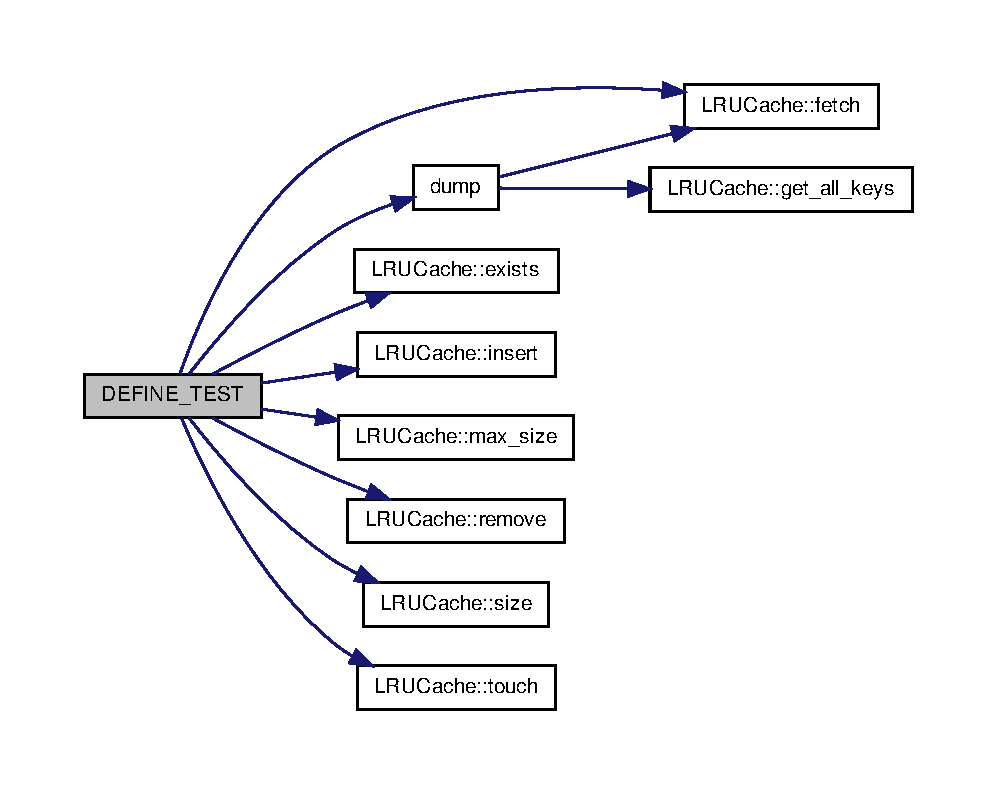
\includegraphics[width=400pt]{lru__cache_8cpp_a744e96854fa4e01ab945ea9ad43b39ca_cgraph}
\end{center}
\end{figure}


\index{lru\_\-cache.cpp@{lru\_\-cache.cpp}!DEFINE\_\-TEST@{DEFINE\_\-TEST}}
\index{DEFINE\_\-TEST@{DEFINE\_\-TEST}!lru_cache.cpp@{lru\_\-cache.cpp}}
\subsubsection[{DEFINE\_\-TEST}]{\setlength{\rightskip}{0pt plus 5cm}DEFINE\_\-TEST (
\begin{DoxyParamCaption}
\item[{lru\_\-cache\_\-stress}]{}
\end{DoxyParamCaption}
)}\label{lru__cache_8cpp_a92b18aa64a57a02c1adc3d1b98924bb5}
\begin{Desc}
\item[{\bf Test}]Insert lots of objects and benchmark the rate. \end{Desc}


Definition at line {\bf 123} of file {\bf lru\_\-cache.cpp}.



References {\bf cputime()}, {\bf LRUCache$<$ Key, Data, Sizefn $>$::insert()}, {\bf print\_\-cputime()}, and {\bf unit\_\-pass}.




\begin{DoxyCode}
                                \{
        \textcolor{comment}{// Stress test the implementation a little more using no objects}
        unit_lru_type2 *L2 = \textcolor{keyword}{new} unit_lru_type2(5);
        \textcolor{keywordtype}{double} t0 = cputime();
        \textcolor{keywordflow}{for}( \textcolor{keywordtype}{int} i = 0; i < TRANSACTIONS; i++ ) \{
                L2->insert( i, i-1 );
        \}
        \textcolor{keywordtype}{double} t1 = cputime();
        \textcolor{keyword}{delete} L2;
        print_cputime( \textcolor{stringliteral}{"(int,int) inserts"}, t1-t0, TRANSACTIONS );
        unit_pass();
\}
\end{DoxyCode}




Here is the call graph for this function:\nopagebreak
\begin{figure}[H]
\begin{center}
\leavevmode
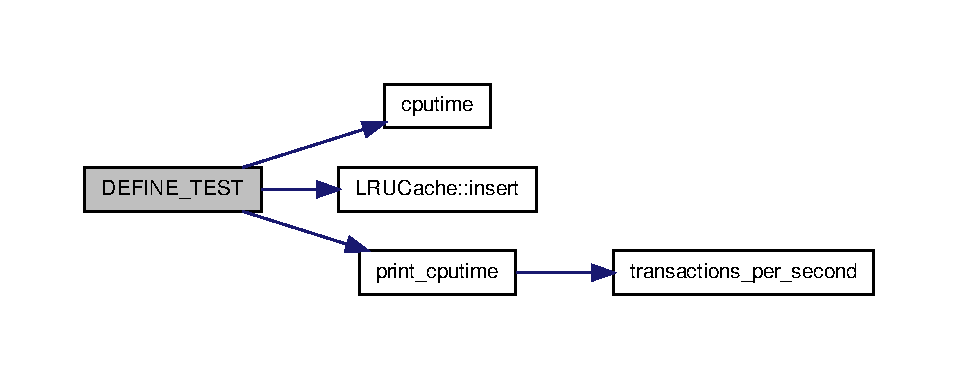
\includegraphics[width=400pt]{lru__cache_8cpp_a92b18aa64a57a02c1adc3d1b98924bb5_cgraph}
\end{center}
\end{figure}


\index{lru\_\-cache.cpp@{lru\_\-cache.cpp}!DEFINE\_\-TEST@{DEFINE\_\-TEST}}
\index{DEFINE\_\-TEST@{DEFINE\_\-TEST}!lru_cache.cpp@{lru\_\-cache.cpp}}
\subsubsection[{DEFINE\_\-TEST}]{\setlength{\rightskip}{0pt plus 5cm}DEFINE\_\-TEST (
\begin{DoxyParamCaption}
\item[{lru\_\-cache\_\-scope\_\-check}]{}
\end{DoxyParamCaption}
)}\label{lru__cache_8cpp_a6288e1898f19682582c52a5005e10ada}
\begin{Desc}
\item[{\bf Test}]Check that objects inserted in a different scope are still there. \end{Desc}


Definition at line {\bf 137} of file {\bf lru\_\-cache.cpp}.



References {\bf LRUCache$<$ Key, Data, Sizefn $>$::fetch\_\-ptr()}, {\bf unit\_\-assert}, and {\bf unit\_\-pass}.




\begin{DoxyCode}
                                     \{
        test\_big\_data* B = L3->fetch_ptr( 9 );
        unit_assert( \textcolor{stringliteral}{"scope check element L3[1]"}, ( strncmp( B->buffer, \textcolor{stringliteral}{"9\(\backslash\)n"}, 10
      00 ) == 0 ) );
        B = L3->fetch_ptr( 8 );
        unit_assert( \textcolor{stringliteral}{"scope check element L3[2]"}, ( strncmp( B->buffer, \textcolor{stringliteral}{"8\(\backslash\)n"}, 10
      00 ) == 0 ) );
        \textcolor{keyword}{delete} L3;
        unit_pass();
\}
\end{DoxyCode}




Here is the call graph for this function:\nopagebreak
\begin{figure}[H]
\begin{center}
\leavevmode
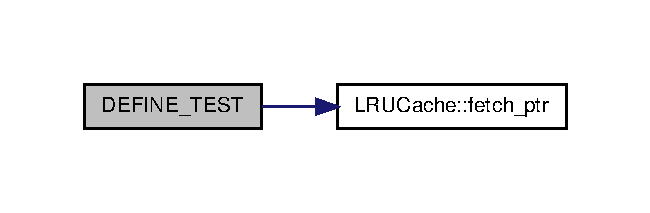
\includegraphics[width=312pt]{lru__cache_8cpp_a6288e1898f19682582c52a5005e10ada_cgraph}
\end{center}
\end{figure}


\index{lru\_\-cache.cpp@{lru\_\-cache.cpp}!DEFINE\_\-TEST@{DEFINE\_\-TEST}}
\index{DEFINE\_\-TEST@{DEFINE\_\-TEST}!lru_cache.cpp@{lru\_\-cache.cpp}}
\subsubsection[{DEFINE\_\-TEST}]{\setlength{\rightskip}{0pt plus 5cm}DEFINE\_\-TEST (
\begin{DoxyParamCaption}
\item[{lru\_\-cache\_\-threads}]{}
\end{DoxyParamCaption}
)}\label{lru__cache_8cpp_a7403186cac9b12671fdda33ea88bceb0}
\begin{Desc}
\item[{\bf Test}]Check for badness with multithreaded access, this is more of a stress test than an empirical test. \end{Desc}


Definition at line {\bf 164} of file {\bf lru\_\-cache.cpp}.



References {\bf cputime()}, {\bf print\_\-cputime()}, and {\bf unit\_\-pass}.




\begin{DoxyCode}
                                 \{
        L4 = \textcolor{keyword}{new} unit_lru_type2( 20 );
        boost::thread\_group thrds;
        \textcolor{keywordtype}{double} t0 = cputime();
        \textcolor{keywordflow}{for} (\textcolor{keywordtype}{int} i=0; i < THREAD\_COUNT; ++i)
                thrds.create\_thread(&insert\_junk);
        thrds.join\_all();
        \textcolor{keywordtype}{double} t1 = cputime();
        print_cputime( \textcolor{stringliteral}{"(int,int) multithreaded inserts"}, t1-t0, THREAD\_TRANS*THR
      EAD\_COUNT*4 );
        \textcolor{keyword}{delete} L4;
        unit_pass();
\}
\end{DoxyCode}




Here is the call graph for this function:\nopagebreak
\begin{figure}[H]
\begin{center}
\leavevmode
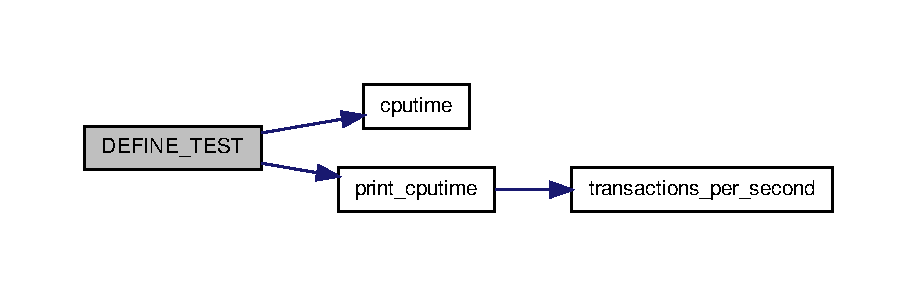
\includegraphics[width=400pt]{lru__cache_8cpp_a7403186cac9b12671fdda33ea88bceb0_cgraph}
\end{center}
\end{figure}



\section{lru\_\-cache.cpp}

\begin{DoxyCode}
00001 \textcolor{comment}{/***************************************************************************}
00002 \textcolor{comment}{ *   Copyright (C) 2004-2011 by Patrick Audley                             *}
00003 \textcolor{comment}{ *   paudley@blackcat.ca                                                   *}
00004 \textcolor{comment}{ *   http://patrickaudley.com                                              *}
00005 \textcolor{comment}{ *                                                                         *}
00006 \textcolor{comment}{ ***************************************************************************/}
00011 \textcolor{preprocessor}{#include "lru_cache.h"}
00012 
00013 \textcolor{preprocessor}{#ifdef UNITTEST}
00014 \textcolor{preprocessor}{}\textcolor{preprocessor}{#include "unit_test.h"}
00015 \textcolor{preprocessor}{#include <string>}
00016 \textcolor{preprocessor}{#include <stdlib.h>}
00017 
00019 \textcolor{keyword}{typedef} LRUCache<std::string,std::string> unit_lru_type;
00021 \textcolor{keyword}{typedef} LRUCache<int,int> unit_lru_type2;
00023 \textcolor{keyword}{class }test\_big\_data \{
00024         \textcolor{keyword}{public}:
00025                 \textcolor{keywordtype}{char} buffer[1000];
00026 \};
00028 \textcolor{keyword}{typedef} LRUCache<int,test_big_data> unit_lru_type3;
00029 
00031 std::string dump( unit_lru_type *L ) \{
00032         unit_lru_type::Key_List \_list( L->get_all_keys() );
00033         std::string ret(\textcolor{stringliteral}{""});
00034         \textcolor{keywordflow}{for}( unit_lru_type::Key_List_Iter liter = \_list.begin(); liter != \_list.e
      nd(); liter++ ) \{
00035                 ret.append( *liter );
00036                 ret.append( \textcolor{stringliteral}{":"} );
00037                 ret.append( L->fetch( *liter, \textcolor{keyword}{false} ) );
00038                 ret.append( \textcolor{stringliteral}{"\(\backslash\)n"} );
00039         \}
00040         \textcolor{comment}{//std::cout << "Dump--" << std::endl << ret << "----" << std::endl;}
00041         \textcolor{keywordflow}{return} ret;
00042 \}
00043 
00045 unit_lru_type3* L3;
00046 
00047 UNIT_TEST_DEFINES
00048 
00050 DEFINE_TEST( lru\_cache\_1cycle ) \{
00051         \textcolor{keyword}{const} std::string unit\_data\_1cycle\_a(\textcolor{stringliteral}{"foo:4\(\backslash\)n"});
00052         \textcolor{keyword}{const} std::string unit\_data\_1cycle\_b(\textcolor{stringliteral}{"bar:flower\(\backslash\)nfoo:4\(\backslash\)n"});
00053         \textcolor{keyword}{const} std::string unit\_data\_1cycle\_c(\textcolor{stringliteral}{"foo:4\(\backslash\)nbar:flower\(\backslash\)n"});
00054         \textcolor{keyword}{const} std::string unit\_data\_1cycle\_d(\textcolor{stringliteral}{"foo:moose\(\backslash\)nbaz:Stalin\(\backslash\)nbar:flower\(\backslash\)n
      "});
00055         \textcolor{keyword}{const} std::string unit\_data\_1cycle\_e(\textcolor{stringliteral}{"foo:moose\(\backslash\)nbar:flower\(\backslash\)n"});
00056         \textcolor{keyword}{const} std::string unit\_data\_1cycle\_f(\textcolor{stringliteral}{"quz:xyzzy\(\backslash\)nbaz:monkey\(\backslash\)nfoo:moose\(\backslash\)n"
      });
00057         \textcolor{keyword}{const} std::string unit\_data\_1cycle\_g(\textcolor{stringliteral}{"coat:mouse\(\backslash\)npants:cat\(\backslash\)nsocks:bear\(\backslash\)n
      "});
00058 
00059         unit_lru_type *L = \textcolor{keyword}{new} unit_lru_type(3);
00060         unit_assert( \textcolor{stringliteral}{"size==0"}, (L->size() == 0) );
00061         unit_assert( \textcolor{stringliteral}{"maxsize==3"}, (L->max_size() == 3) );
00062 
00063         \textcolor{comment}{// Checking a bogus key shouldn't alter the cache.}
00064         L->exists( \textcolor{stringliteral}{"foo"} );
00065         unit_assert( \textcolor{stringliteral}{"exists() doesn't increase size"}, (L->size() == 0) );
00066 
00067         \textcolor{comment}{// Check insert() and exists()}
00068         L->insert( \textcolor{stringliteral}{"foo"}, \textcolor{stringliteral}{"4"} );
00069         unit_assert( \textcolor{stringliteral}{"size==1 after insert(foo,4)"}, (L->size() == 1) );
00070         unit_assert( \textcolor{stringliteral}{"check exists(foo)"}, L->exists( \textcolor{stringliteral}{"foo"} ) );
00071         unit_assert( \textcolor{stringliteral}{"contents check a)"}, unit\_data\_1cycle\_a.compare( dump( L ) )
       == 0 );
00072 
00073         \textcolor{comment}{// Check second insert and ordering}
00074         L->insert( \textcolor{stringliteral}{"bar"}, \textcolor{stringliteral}{"flower"} );
00075         unit_assert( \textcolor{stringliteral}{"size==2 after insert(bar,flower)"}, (L->size() == 2) );
00076         unit_assert( \textcolor{stringliteral}{"contents check b)"}, unit\_data\_1cycle\_b.compare( dump( L ) )
       == 0 );
00077 
00078         \textcolor{comment}{// Check touching}
00079         L->touch( \textcolor{stringliteral}{"foo"} );
00080         unit_assert( \textcolor{stringliteral}{"contents check c)"}, unit\_data\_1cycle\_c.compare( dump( L ) )
       == 0 );
00081 
00082         \textcolor{comment}{// Insert of an existing element should result in only a touch}
00083         L->insert( \textcolor{stringliteral}{"bar"}, \textcolor{stringliteral}{"flower"} );
00084         unit_assert( \textcolor{stringliteral}{"verify insert touches"}, unit\_data\_1cycle\_b.compare( dump( L
       ) ) == 0 );
00085 
00086         \textcolor{comment}{// Verify that fetch works}
00087         unit_assert( \textcolor{stringliteral}{"verify fetch(bar)"}, ( std::string(\textcolor{stringliteral}{"flower"}).compare( L->
      fetch(\textcolor{stringliteral}{"bar"}) ) == 0 ) );
00088 
00089         \textcolor{comment}{// Insert of an existing element with new data should replace and touch}
00090         L->insert( \textcolor{stringliteral}{"baz"}, \textcolor{stringliteral}{"Stalin"} );
00091         L->insert( \textcolor{stringliteral}{"foo"}, \textcolor{stringliteral}{"moose"} );
00092         unit_assert( \textcolor{stringliteral}{"verify insert replaces"}, unit\_data\_1cycle\_d.compare( dump( 
      L ) ) == 0 );
00093 
00094         \textcolor{comment}{// Test removal of an existing member.}
00095         L->remove( \textcolor{stringliteral}{"baz"} );
00096         unit_assert( \textcolor{stringliteral}{"verify remove works"}, unit\_data\_1cycle\_e.compare( dump( L )
       ) == 0 );
00097 
00098         \textcolor{comment}{// Test LRU removal as we add more members than max\_size()}
00099         L->insert( \textcolor{stringliteral}{"baz"}, \textcolor{stringliteral}{"monkey"} );
00100         L->insert( \textcolor{stringliteral}{"quz"}, \textcolor{stringliteral}{"xyzzy"} );
00101         unit_assert( \textcolor{stringliteral}{"verify LRU semantics"}, unit\_data\_1cycle\_f.compare( dump( L 
      ) ) == 0 );
00102 
00103         \textcolor{comment}{// Stress test the implementation a little..}
00104         \textcolor{keyword}{const} \textcolor{keywordtype}{char} *names[10] = \{ \textcolor{stringliteral}{"moose"}, \textcolor{stringliteral}{"dog"}, \textcolor{stringliteral}{"bear"}, \textcolor{stringliteral}{"cat"}, \textcolor{stringliteral}{"mouse"}, \textcolor{stringliteral}{"hat"}, 
      \textcolor{stringliteral}{"mittens"}, \textcolor{stringliteral}{"socks"}, \textcolor{stringliteral}{"pants"}, \textcolor{stringliteral}{"coat"} \};
00105         \textcolor{keywordflow}{for}( \textcolor{keywordtype}{int} i = 0; i < 50; i++ ) \{
00106                 L->insert( names[ i % 10 ], names[ i % 9 ] );
00107         \}
00108         unit_assert( \textcolor{stringliteral}{"stress test a little"}, unit\_data\_1cycle\_g.compare( dump( L 
      ) ) == 0 );
00109 
00110         \textcolor{comment}{// Setup a little for the third test which verifies that scoped reference
      s inserted into the cache don't disappear.}
00111         L3 = \textcolor{keyword}{new} unit_lru_type3(2);
00112         \textcolor{keywordflow}{for}( \textcolor{keywordtype}{int} i = 0; i < 10; i++ ) \{
00113                 test\_big\_data B;
00114                 snprintf( B.buffer, 1000, \textcolor{stringliteral}{"%d\(\backslash\)n"}, i );
00115                 L3->insert( i, B );
00116         \}
00117 
00118         unit_pass();
00119 \}
00120 
00121 \textcolor{preprocessor}{#define TRANSACTIONS 50000}
00122 \textcolor{preprocessor}{}
00123 DEFINE_TEST( lru\_cache\_stress ) \{
00124         \textcolor{comment}{// Stress test the implementation a little more using no objects}
00125         unit_lru_type2 *L2 = \textcolor{keyword}{new} unit_lru_type2(5);
00126         \textcolor{keywordtype}{double} t0 = cputime();
00127         \textcolor{keywordflow}{for}( \textcolor{keywordtype}{int} i = 0; i < TRANSACTIONS; i++ ) \{
00128                 L2->insert( i, i-1 );
00129         \}
00130         \textcolor{keywordtype}{double} t1 = cputime();
00131         \textcolor{keyword}{delete} L2;
00132         print_cputime( \textcolor{stringliteral}{"(int,int) inserts"}, t1-t0, TRANSACTIONS );
00133         unit_pass();
00134 \}
00135 
00137 DEFINE_TEST( lru\_cache\_scope\_check ) \{
00138         test\_big\_data* B = L3->fetch_ptr( 9 );
00139         unit_assert( \textcolor{stringliteral}{"scope check element L3[1]"}, ( strncmp( B->buffer, \textcolor{stringliteral}{"9\(\backslash\)n"}, 10
      00 ) == 0 ) );
00140         B = L3->fetch_ptr( 8 );
00141         unit_assert( \textcolor{stringliteral}{"scope check element L3[2]"}, ( strncmp( B->buffer, \textcolor{stringliteral}{"8\(\backslash\)n"}, 10
      00 ) == 0 ) );
00142         \textcolor{keyword}{delete} L3;
00143         unit_pass();
00144 \}
00145 
00146 \textcolor{preprocessor}{#ifdef \_REENTRANT}
00147 \textcolor{preprocessor}{}\textcolor{preprocessor}{#include <boost/thread/thread.hpp>}
00148 
00149 \textcolor{preprocessor}{#define THREAD\_TRANS 20000}
00150 \textcolor{preprocessor}{}\textcolor{preprocessor}{#define THREAD\_COUNT 10}
00151 \textcolor{preprocessor}{}
00152 unit_lru_type2 *L4;
00153 
00154 \textcolor{keywordtype}{void} insert\_junk()\{
00155         \textcolor{keywordflow}{for}( \textcolor{keywordtype}{int} i = 0; i < THREAD\_TRANS; i++ ) \{
00156                 L4->insert( i, i+1 );
00157                 L4->remove( i-5 );
00158                 L4->fetch( i-3 );
00159                 L4->touch( i-10 );
00160         \}
00161 \}
00162 
00164 DEFINE_TEST( lru\_cache\_threads ) \{
00165         L4 = \textcolor{keyword}{new} unit_lru_type2( 20 );
00166         boost::thread\_group thrds;
00167         \textcolor{keywordtype}{double} t0 = cputime();
00168         \textcolor{keywordflow}{for} (\textcolor{keywordtype}{int} i=0; i < THREAD\_COUNT; ++i)
00169                 thrds.create\_thread(&insert\_junk);
00170         thrds.join\_all();
00171         \textcolor{keywordtype}{double} t1 = cputime();
00172         print_cputime( \textcolor{stringliteral}{"(int,int) multithreaded inserts"}, t1-t0, THREAD\_TRANS*THR
      EAD\_COUNT*4 );
00173         \textcolor{keyword}{delete} L4;
00174         unit_pass();
00175 \}
00176 
00177 \textcolor{preprocessor}{#endif}
00178 \textcolor{preprocessor}{}
00179 UNIT_TEST_RUN( \textcolor{stringliteral}{"LRU Cache"} );
00180         ADD_TEST( lru\_cache\_1cycle );
00181         ADD_TEST( lru\_cache\_stress );
00182         ADD_TEST( lru\_cache\_scope\_check );
00183 \textcolor{preprocessor}{#ifdef \_REENTRANT}
00184 \textcolor{preprocessor}{}        ADD_TEST( lru\_cache\_threads );
00185 \textcolor{preprocessor}{#endif}
00186 \textcolor{preprocessor}{}UNIT\_TEST\_END;
00187 
00188 \textcolor{preprocessor}{#endif}
\end{DoxyCode}

\section{lru\_\-cache.h File Reference}
\label{lru__cache_8h}\index{lru\_\-cache.h@{lru\_\-cache.h}}
\subsection*{Classes}
\begin{DoxyCompactItemize}
\item 
class {\bf LRUCache$<$ Key, Data, Sizefn $>$}
\begin{DoxyCompactList}\small\item\em Template cache with an LRU removal policy. \item\end{DoxyCompactList}\end{DoxyCompactItemize}
\subsection*{Defines}
\begin{DoxyCompactItemize}
\item 
\#define {\bf SCOPED\_\-MUTEX}~boost::mutex::scoped\_\-lock lock(this-\/$>$\_\-mutex);\label{lru__cache_8h_a7a1d17c8eef1fd310a6522744483ae52}

\begin{DoxyCompactList}\small\item\em If we are reentrant then use a BOOST scoped mutex where neccessary. \item\end{DoxyCompactList}\end{DoxyCompactItemize}


\subsection{Detailed Description}
Template cache with an LRU removal policy \begin{DoxyAuthor}{Author}
Patrick Audley 
\end{DoxyAuthor}
\begin{DoxyVersion}{Version}
1.3 
\end{DoxyVersion}
\begin{DoxyDate}{Date}
May 2011 
\end{DoxyDate}
\begin{DoxyParagraph}{}
This cache is thread safe if compiled with \_\-REENTRANT defined. It uses the BOOST scientific computing library to provide the thread safety mutexes.
\end{DoxyParagraph}
\begin{DoxyParagraph}{}
Thanks to {\tt graydon@pobox.com} for the size counting functor. 
\end{DoxyParagraph}


Definition in file {\bf lru\_\-cache.h}.


\section{lru\_\-cache.h}

\begin{DoxyCode}
00001 \textcolor{comment}{/***************************************************************************}
00002 \textcolor{comment}{ *   Copyright (C) 2004-2011 by Patrick Audley                             *}
00003 \textcolor{comment}{ *   paudley@blackcat.ca                                                   *}
00004 \textcolor{comment}{ *   http://patrickaudley.com                                              *}
00005 \textcolor{comment}{ *                                                                         *}
00006 \textcolor{comment}{ ***************************************************************************/}
00045 \textcolor{preprocessor}{#include <map>}
00046 \textcolor{preprocessor}{#include <list>}
00047 \textcolor{preprocessor}{#include <vector>}
00048 \textcolor{preprocessor}{#ifdef \_REENTRANT}
00049 \textcolor{preprocessor}{}\textcolor{preprocessor}{#include <boost/thread/mutex.hpp>}
00051 \textcolor{preprocessor}{#define SCOPED\_MUTEX  boost::mutex::scoped\_lock lock(this->\_mutex);}
00052 \textcolor{preprocessor}{}\textcolor{preprocessor}{#else}
00053 \textcolor{preprocessor}{}
00054 \textcolor{preprocessor}{#define SCOPED\_MUTEX}
00055 \textcolor{preprocessor}{}\textcolor{preprocessor}{#endif}
00056 \textcolor{preprocessor}{}
00057 \textcolor{keyword}{template} < \textcolor{keyword}{class} T >
00058 \textcolor{keyword}{struct }Countfn \{
00059                 \textcolor{keywordtype}{unsigned} \textcolor{keywordtype}{long} operator()( \textcolor{keyword}{const} T &x ) \{ \textcolor{keywordflow}{return} 1; \}
00060 \};
00061 
00062 
00073 \textcolor{keyword}{template}< \textcolor{keyword}{class} Key, \textcolor{keyword}{class} Data, \textcolor{keyword}{class} Sizefn = Countfn< Data > > \textcolor{keyword}{class }LRUCache 
      \{
00074         \textcolor{keyword}{public}:
00075                 \textcolor{keyword}{typedef} std::list< std::pair< Key, Data > > List;         
00076                 \textcolor{keyword}{typedef} \textcolor{keyword}{typename} List::iterator List\_Iter;                
00077                 \textcolor{keyword}{typedef} \textcolor{keyword}{typename} List::const\_iterator List\_cIter;         
00078                 \textcolor{keyword}{typedef} std::vector< Key > Key\_List;                      
00079                 \textcolor{keyword}{typedef} \textcolor{keyword}{typename} Key\_List::iterator Key\_List\_Iter;        
00080                 \textcolor{keyword}{typedef} \textcolor{keyword}{typename} Key\_List::const\_iterator Key\_List\_cIter; 
00081                 \textcolor{keyword}{typedef} std::map< Key, List\_Iter > Map;                   
00082                 \textcolor{keyword}{typedef} std::pair< Key, List\_Iter > Pair;                 
00083                 \textcolor{keyword}{typedef} \textcolor{keyword}{typename} Map::iterator Map\_Iter;                         
                 
00084                 \textcolor{keyword}{typedef} \textcolor{keyword}{typename} Map::const\_iterator Map\_cIter;           
00085 
00086         \textcolor{keyword}{private}:
00087                 List \_list;               
00088                 Map \_index;               
00089                 \textcolor{keywordtype}{unsigned} \textcolor{keywordtype}{long} \_max\_size;  
00090                 \textcolor{keywordtype}{unsigned} \textcolor{keywordtype}{long} \_curr\_size; 
00091 
00092 \textcolor{preprocessor}{#ifdef \_REENTRANT}
00093 \textcolor{preprocessor}{}                boost::mutex \_mutex;
00094 \textcolor{preprocessor}{#endif}
00095 \textcolor{preprocessor}{}
00096         \textcolor{keyword}{public}:
00097 
00101                 LRUCache( \textcolor{keyword}{const} \textcolor{keywordtype}{unsigned} \textcolor{keywordtype}{long} Size ) :
00102                                 \_max\_size( Size ),
00103                                 \_curr\_size( 0 )
00104                                 \{\}
00105 
00107                 ~LRUCache() \{ clear(); \}
00108 
00112                 \textcolor{keyword}{inline} \textcolor{keyword}{const} \textcolor{keywordtype}{unsigned} \textcolor{keywordtype}{long} size( \textcolor{keywordtype}{void} )\textcolor{keyword}{ const }\{ \textcolor{keywordflow}{return} \_curr\_size
      ; \}
00113 
00117                 \textcolor{keyword}{inline} \textcolor{keyword}{const} \textcolor{keywordtype}{unsigned} \textcolor{keywordtype}{long} max_size( \textcolor{keywordtype}{void} )\textcolor{keyword}{ const }\{ \textcolor{keywordflow}{return} \_max\_s
      ize; \}
00118 
00120                 \textcolor{keywordtype}{void} clear( \textcolor{keywordtype}{void} ) \{
00121                         SCOPED\_MUTEX;
00122                         \_list.clear();
00123                         \_index.clear();
00124                 \};
00125 
00130 \textcolor{preprocessor}{#ifdef \_REENTRANT}
00131 \textcolor{preprocessor}{}                \textcolor{keyword}{inline} \textcolor{keywordtype}{bool} exists( \textcolor{keyword}{const} Key &key ) \{
00132                         SCOPED\_MUTEX;
00133 \textcolor{preprocessor}{#else}
00134 \textcolor{preprocessor}{}                \textcolor{keyword}{inline} \textcolor{keywordtype}{bool} exists( \textcolor{keyword}{const} Key &key )\textcolor{keyword}{ const }\{
00135 \textcolor{preprocessor}{#endif}
00136 \textcolor{preprocessor}{}                        \textcolor{keywordflow}{return} \_index.find( key ) != \_index.end();
00137                 \}
00138 
00142                 \textcolor{keyword}{inline} \textcolor{keywordtype}{void} \textcolor{keyword}{remove}( \textcolor{keyword}{const} Key &key ) \{
00143 \textcolor{preprocessor}{#ifdef \_REENTRANT}
00144 \textcolor{preprocessor}{}                        SCOPED\_MUTEX;
00145 \textcolor{preprocessor}{#endif}
00146 \textcolor{preprocessor}{}                        Map_Iter miter = \_index.find( key );
00147                         \textcolor{keywordflow}{if}( miter == \_index.end() ) \textcolor{keywordflow}{return};
00148                         \_remove( miter );
00149                 \}
00150 
00154                 \textcolor{keyword}{inline} \textcolor{keywordtype}{void} touch( \textcolor{keyword}{const} Key &key ) \{
00155                         SCOPED\_MUTEX;
00156                         \_touch( key );
00157                 \}
00158 
00164                 \textcolor{keyword}{inline} Data *fetch_ptr( \textcolor{keyword}{const} Key &key, \textcolor{keywordtype}{bool} touch = \textcolor{keyword}{true} ) \{
00165                         SCOPED\_MUTEX;
00166                         Map_Iter miter = \_index.find( key );
00167                         \textcolor{keywordflow}{if}( miter == \_index.end() ) \textcolor{keywordflow}{return} NULL;
00168                         \_touch( key );
00169                         \textcolor{keywordflow}{return} &(miter->second->second);
00170                 \}
00171 
00177                 \textcolor{keyword}{inline} Data fetch( \textcolor{keyword}{const} Key &key, \textcolor{keywordtype}{bool} touch\_data = \textcolor{keyword}{true} ) \{
00178                         SCOPED\_MUTEX;
00179                         Map_Iter miter = \_index.find( key );
00180                         \textcolor{keywordflow}{if}( miter == \_index.end() )
00181                                 \textcolor{keywordflow}{return} Data();
00182                         Data tmp = miter->second->second;
00183                         \textcolor{keywordflow}{if}( touch\_data )
00184                                 \_touch( key );
00185                         \textcolor{keywordflow}{return} tmp;
00186                 \}
00187 
00194                 \textcolor{keyword}{inline} \textcolor{keywordtype}{bool} fetch( \textcolor{keyword}{const} Key &key, Data &data, \textcolor{keywordtype}{bool} touch\_data = 
      \textcolor{keyword}{true} ) \{
00195                         SCOPED\_MUTEX;
00196                         Map_Iter miter = \_index.find( key );
00197                         \textcolor{keywordflow}{if}( miter == \_index.end() ) \textcolor{keywordflow}{return} \textcolor{keyword}{false};
00198                         \textcolor{keywordflow}{if}( touch\_data )
00199                           \_touch( key );
00200                         data = miter->second->second;
00201                         \textcolor{keywordflow}{return} \textcolor{keyword}{true};
00202                 \}
00203 
00209                 \textcolor{keyword}{inline} \textcolor{keywordtype}{void} insert( \textcolor{keyword}{const} Key &key, \textcolor{keyword}{const} Data &data ) \{
00210                         SCOPED\_MUTEX;
00211                         \textcolor{comment}{// Touch the key, if it exists, then replace the content.
      }
00212                         Map_Iter miter = \_touch( key );
00213                         \textcolor{keywordflow}{if}( miter != \_index.end() )
00214                                 \_remove( miter );
00215 
00216                         \textcolor{comment}{// Ok, do the actual insert at the head of the list}
00217                         \_list.push\_front( std::make\_pair( key, data ) );
00218                         List_Iter liter = \_list.begin();
00219 
00220                         \textcolor{comment}{// Store the index}
00221                         \_index.insert( std::make\_pair( key, liter ) );
00222                         \_curr\_size += Sizefn()( data );
00223 
00224                         \textcolor{comment}{// Check to see if we need to remove an element due to ex
      ceeding max\_size}
00225                         \textcolor{keywordflow}{while}( \_curr\_size > \_max\_size ) \{
00226                                 \textcolor{comment}{// Remove the last element.}
00227                                 liter = \_list.end();
00228                                 --liter;
00229                                 \_remove( liter->first );
00230                         \}
00231                 \}
00232 
00236                 \textcolor{keyword}{inline} \textcolor{keyword}{const} Key_List get_all_keys( \textcolor{keywordtype}{void} ) \{
00237                         SCOPED\_MUTEX;
00238                         Key_List ret;
00239                         \textcolor{keywordflow}{for}( List_cIter liter = \_list.begin(); liter != \_list.end
      (); liter++ )
00240                                 ret.push\_back( liter->first );
00241                         \textcolor{keywordflow}{return} ret;
00242                 \}
00243 
00244         \textcolor{keyword}{private}:
00249                 \textcolor{keyword}{inline} Map_Iter \_touch( \textcolor{keyword}{const} Key &key ) \{
00250                         Map_Iter miter = \_index.find( key );
00251                         \textcolor{keywordflow}{if}( miter == \_index.end() ) \textcolor{keywordflow}{return} miter;
00252                         \textcolor{comment}{// Move the found node to the head of the list.}
00253                         \_list.splice( \_list.begin(), \_list, miter->second );
00254                         \textcolor{keywordflow}{return} miter;
00255                 \}
00256 
00261                 \textcolor{keyword}{inline} \textcolor{keywordtype}{void} \_remove( \textcolor{keyword}{const} Map_Iter &miter ) \{
00262                         \_curr\_size -= Sizefn()( miter->second->second );
00263                         \_list.erase( miter->second );
00264                         \_index.erase( miter );
00265                 \}
00266 
00270                 \textcolor{keyword}{inline} \textcolor{keywordtype}{void} \_remove( \textcolor{keyword}{const} Key &key ) \{
00271                         Map_Iter miter = \_index.find( key );
00272                         \_remove( miter );
00273                 \}
00274 \};
\end{DoxyCode}

\section{unit\_\-test.h File Reference}
\label{unit__test_8h}\index{unit\_\-test.h@{unit\_\-test.h}}
\subsection*{Defines}
\begin{DoxyCompactItemize}
\item 
\#define {\bf UNIT\_\-TEST\_\-DEFINES}\label{unit__test_8h_a5f3fe0e0e85d0dc03672f96e5e95856f}

\begin{DoxyCompactList}\small\item\em Start of inline Unit Test definitions Use this to start the list of unit tests. This should be followed by one or more DEFINE\_\-TEST entries. \item\end{DoxyCompactList}\item 
\#define {\bf DEFINE\_\-TEST}(test\_\-name)~bool unit\_\-test\_\-\#\#test\_\-name (void)
\begin{DoxyCompactList}\small\item\em Start a new test definition. \item\end{DoxyCompactList}\item 
\#define {\bf ADD\_\-TEST}(test\_\-name)~add\_\-test( \&unit\_\-test\_\-\#\#test\_\-name );
\begin{DoxyCompactList}\small\item\em Adds a defined test to test run. \item\end{DoxyCompactList}\item 
\#define {\bf UNIT\_\-TEST\_\-RUN}(suite)
\begin{DoxyCompactList}\small\item\em Start a Unit test run section. \item\end{DoxyCompactList}\item 
\#define {\bf unit\_\-assert}(msg, cond)
\begin{DoxyCompactList}\small\item\em Use within a Unit Test to verify a condition. \item\end{DoxyCompactList}\item 
\#define {\bf unit\_\-pass}()~return true;
\begin{DoxyCompactList}\small\item\em Use to end a unit test in success. \item\end{DoxyCompactList}\item 
\#define {\bf unit\_\-fail}()~return false;
\begin{DoxyCompactList}\small\item\em Use to end a unit test in failure. \item\end{DoxyCompactList}\item 
\#define {\bf UNIT\_\-TEST\_\-END}\label{unit__test_8h_a732dd1ba2cfc9163d60e05628b4544dc}

\begin{DoxyCompactList}\small\item\em Finish a Unit Test run section. \item\end{DoxyCompactList}\end{DoxyCompactItemize}
\subsection*{Typedefs}
\begin{DoxyCompactItemize}
\item 
typedef bool($\ast$ {\bf test\_\-func} )(void)\label{unit__test_8h_a62a6058fdd96dcd306fba96626b2cc71}

\begin{DoxyCompactList}\small\item\em typedef for unittest functions \item\end{DoxyCompactList}\item 
typedef std::vector$<$ {\bf test\_\-func} $>$ {\bf test\_\-vector}\label{unit__test_8h_a76894e75beeadd2872f2f5909b43e36f}

\begin{DoxyCompactList}\small\item\em typedef for vectors of unittest functions \item\end{DoxyCompactList}\end{DoxyCompactItemize}
\subsection*{Functions}
\begin{DoxyCompactItemize}
\item 
double {\bf cputime} (void)
\begin{DoxyCompactList}\small\item\em Gets the current CPU time with microsecond accuracy. \item\end{DoxyCompactList}\item 
double {\bf transactions\_\-per\_\-second} (double run\_\-time, unsigned long transactions)
\begin{DoxyCompactList}\small\item\em Calculates the transactions rate. \item\end{DoxyCompactList}\item 
void {\bf print\_\-cputime} (const char $\ast$msg, double run\_\-time, unsigned long transactions=0)
\begin{DoxyCompactList}\small\item\em Prints to stdout the results of timing an event. \item\end{DoxyCompactList}\end{DoxyCompactItemize}


\subsection{Detailed Description}
Unit Testing framework for C++ \begin{DoxyAuthor}{Author}
Patrick Audley 
\end{DoxyAuthor}
\begin{DoxyDate}{Date}
December 2004
\end{DoxyDate}
\begin{DoxyParagraph}{}
See full documentation for this framework in \doxyref{Unit Testing Framework}{p.}{unittests01} 
\end{DoxyParagraph}


Definition in file {\bf unit\_\-test.h}.



\subsection{Define Documentation}
\index{unit\_\-test.h@{unit\_\-test.h}!DEFINE\_\-TEST@{DEFINE\_\-TEST}}
\index{DEFINE\_\-TEST@{DEFINE\_\-TEST}!unit_test.h@{unit\_\-test.h}}
\subsubsection[{DEFINE\_\-TEST}]{\setlength{\rightskip}{0pt plus 5cm}\#define DEFINE\_\-TEST(
\begin{DoxyParamCaption}
\item[{}]{test\_\-name}
\end{DoxyParamCaption}
)~bool unit\_\-test\_\-\#\#test\_\-name (void)}\label{unit__test_8h_ad3bccea4c3142d58fd5510f65503b300}


Start a new test definition. 


\begin{DoxyParams}{Parameters}
\item[{\em test\_\-name}]Name of the test -\/ must be unique in this unit test suite. \end{DoxyParams}


Definition at line {\bf 184} of file {\bf unit\_\-test.h}.

\index{unit\_\-test.h@{unit\_\-test.h}!ADD\_\-TEST@{ADD\_\-TEST}}
\index{ADD\_\-TEST@{ADD\_\-TEST}!unit_test.h@{unit\_\-test.h}}
\subsubsection[{ADD\_\-TEST}]{\setlength{\rightskip}{0pt plus 5cm}\#define ADD\_\-TEST(
\begin{DoxyParamCaption}
\item[{}]{test\_\-name}
\end{DoxyParamCaption}
)~add\_\-test( \&unit\_\-test\_\-\#\#test\_\-name );}\label{unit__test_8h_a758baec4c57fa6aeaf800e2c631a7d9f}


Adds a defined test to test run. 


\begin{DoxyParams}{Parameters}
\item[{\em test\_\-name}]Test name of a previously defined test to add the the current suite. \end{DoxyParams}
\begin{DoxySeeAlso}{See also}
\doxyref{DEFINE\_\-TEST}{p.}{lru__cache_8cpp_a7403186cac9b12671fdda33ea88bceb0} \doxyref{UNIT\_\-TEST\_\-RUN}{p.}{unit__test_8h_a86b577b8af9cc6df174dc0e2e292c365} This should be called after \doxyref{UNIT\_\-TEST\_\-RUN}{p.}{unit__test_8h_a86b577b8af9cc6df174dc0e2e292c365} for each defined test. 
\end{DoxySeeAlso}


Definition at line {\bf 191} of file {\bf unit\_\-test.h}.

\index{unit\_\-test.h@{unit\_\-test.h}!UNIT\_\-TEST\_\-RUN@{UNIT\_\-TEST\_\-RUN}}
\index{UNIT\_\-TEST\_\-RUN@{UNIT\_\-TEST\_\-RUN}!unit_test.h@{unit\_\-test.h}}
\subsubsection[{UNIT\_\-TEST\_\-RUN}]{\setlength{\rightskip}{0pt plus 5cm}\#define UNIT\_\-TEST\_\-RUN(
\begin{DoxyParamCaption}
\item[{}]{suite}
\end{DoxyParamCaption}
)}\label{unit__test_8h_a86b577b8af9cc6df174dc0e2e292c365}
{\bfseries Value:}
\begin{DoxyCode}
\textcolor{keywordtype}{int} main(\textcolor{keywordtype}{void}) \{ \(\backslash\)
  \textcolor{keywordtype}{bool} result = \textcolor{keyword}{true}; \(\backslash\)
  std::cout << \textcolor{stringliteral}{"---[ "} << suite << \textcolor{stringliteral}{" ]--- "} << std::endl;
\end{DoxyCode}


Start a Unit test run section. 


\begin{DoxyParams}{Parameters}
\item[{\em suite}]Name for this test suite. \end{DoxyParams}
\begin{DoxyNote}{Note}
Must be terminated with an UNIT\_\-TEST\_\-END statement. 
\end{DoxyNote}


Definition at line {\bf 197} of file {\bf unit\_\-test.h}.

\index{unit\_\-test.h@{unit\_\-test.h}!unit\_\-assert@{unit\_\-assert}}
\index{unit\_\-assert@{unit\_\-assert}!unit_test.h@{unit\_\-test.h}}
\subsubsection[{unit\_\-assert}]{\setlength{\rightskip}{0pt plus 5cm}\#define unit\_\-assert(
\begin{DoxyParamCaption}
\item[{}]{msg, }
\item[{}]{cond}
\end{DoxyParamCaption}
)}\label{unit__test_8h_aa37d553e7d644c165c888bed8908de20}
{\bfseries Value:}
\begin{DoxyCode}
std::cout << \textcolor{stringliteral}{"  "} << msg << \textcolor{stringliteral}{": "} << std::flush; \(\backslash\)
  \textcolor{keywordflow}{if}( !cond ) \{ std::cout << \textcolor{stringliteral}{"FAILED"} << std::endl; \textcolor{keywordflow}{return} \textcolor{keyword}{false}; \} \(\backslash\)
  std::cout << \textcolor{stringliteral}{"PASSED"} << std::endl;
\end{DoxyCode}


Use within a Unit Test to verify a condition. 

\begin{DoxyWarning}{Warning}
Terminates test on failure. 
\end{DoxyWarning}


Definition at line {\bf 205} of file {\bf unit\_\-test.h}.



Referenced by {\bf DEFINE\_\-TEST()}.

\index{unit\_\-test.h@{unit\_\-test.h}!unit\_\-pass@{unit\_\-pass}}
\index{unit\_\-pass@{unit\_\-pass}!unit_test.h@{unit\_\-test.h}}
\subsubsection[{unit\_\-pass}]{\setlength{\rightskip}{0pt plus 5cm}\#define unit\_\-pass(
\begin{DoxyParamCaption}
{}
\end{DoxyParamCaption}
)~return true;}\label{unit__test_8h_aa2a4504968cf4e8abfc7b706106d4084}


Use to end a unit test in success. 

\begin{DoxyNote}{Note}
Either unit\_\-pass or unit\_\-fail should end every test. 
\end{DoxyNote}


Definition at line {\bf 213} of file {\bf unit\_\-test.h}.



Referenced by {\bf DEFINE\_\-TEST()}.

\index{unit\_\-test.h@{unit\_\-test.h}!unit\_\-fail@{unit\_\-fail}}
\index{unit\_\-fail@{unit\_\-fail}!unit_test.h@{unit\_\-test.h}}
\subsubsection[{unit\_\-fail}]{\setlength{\rightskip}{0pt plus 5cm}\#define unit\_\-fail(
\begin{DoxyParamCaption}
{}
\end{DoxyParamCaption}
)~return false;}\label{unit__test_8h_a3476c32ea638214246ee65f561b6358b}


Use to end a unit test in failure. 

\begin{DoxyNote}{Note}
Either unit\_\-pass or unit\_\-fail should end every test. 
\end{DoxyNote}


Definition at line {\bf 218} of file {\bf unit\_\-test.h}.



\subsection{Function Documentation}
\index{unit\_\-test.h@{unit\_\-test.h}!cputime@{cputime}}
\index{cputime@{cputime}!unit_test.h@{unit\_\-test.h}}
\subsubsection[{cputime}]{\setlength{\rightskip}{0pt plus 5cm}double cputime (
\begin{DoxyParamCaption}
\item[{void}]{}
\end{DoxyParamCaption}
)\hspace{0.3cm}{\ttfamily  [inline]}}\label{unit__test_8h_a7f0155f7ecefd56c2380285420e85e05}


Gets the current CPU time with microsecond accuracy. 

\begin{DoxyReturn}{Returns}
microseconds since UNIX epoch 
\end{DoxyReturn}


Definition at line {\bf 139} of file {\bf unit\_\-test.h}.



Referenced by {\bf DEFINE\_\-TEST()}.




\begin{DoxyCode}
                              \{
  getrusage( RUSAGE\_SELF, &ruse );
        \textcolor{keywordflow}{return} ( ruse.ru\_utime.tv\_sec + ruse.ru\_stime.tv\_sec + 1e-6 * (ruse.ru\_ut
      ime.tv\_usec + ruse.ru\_stime.tv\_usec ) );
\}
\end{DoxyCode}


\index{unit\_\-test.h@{unit\_\-test.h}!transactions\_\-per\_\-second@{transactions\_\-per\_\-second}}
\index{transactions\_\-per\_\-second@{transactions\_\-per\_\-second}!unit_test.h@{unit\_\-test.h}}
\subsubsection[{transactions\_\-per\_\-second}]{\setlength{\rightskip}{0pt plus 5cm}double transactions\_\-per\_\-second (
\begin{DoxyParamCaption}
\item[{double}]{ run\_\-time, }
\item[{unsigned long}]{ transactions}
\end{DoxyParamCaption}
)\hspace{0.3cm}{\ttfamily  [inline]}}\label{unit__test_8h_abf6a6c3c73f9e087ad15d8ed0ec0ba85}


Calculates the transactions rate. 


\begin{DoxyParams}{Parameters}
\item[{\em run\_\-time}]microsecond resolution run time \item[{\em transactions}]number of transactions handled in run\_\-time seconds This is useful if you want to guarantee minimun transactional throughputs in unit tests. \end{DoxyParams}
\begin{DoxyWarning}{Warning}
This code is obviously very test platform dependent. 
\end{DoxyWarning}


Definition at line {\bf 149} of file {\bf unit\_\-test.h}.



Referenced by {\bf print\_\-cputime()}.




\begin{DoxyCode}
                                                                                 
          \{
        \textcolor{keywordflow}{return} (\textcolor{keywordtype}{double})transactions / run\_time;
\}
\end{DoxyCode}


\index{unit\_\-test.h@{unit\_\-test.h}!print\_\-cputime@{print\_\-cputime}}
\index{print\_\-cputime@{print\_\-cputime}!unit_test.h@{unit\_\-test.h}}
\subsubsection[{print\_\-cputime}]{\setlength{\rightskip}{0pt plus 5cm}void print\_\-cputime (
\begin{DoxyParamCaption}
\item[{const char $\ast$}]{ msg, }
\item[{double}]{ run\_\-time, }
\item[{unsigned long}]{ transactions = {\ttfamily 0}}
\end{DoxyParamCaption}
)\hspace{0.3cm}{\ttfamily  [inline]}}\label{unit__test_8h_a2fdd86314c7b39ab4274a36655e833f1}


Prints to stdout the results of timing an event. 


\begin{DoxyParams}{Parameters}
\item[{\em msg}]to print with the numbers \item[{\em run\_\-time}]microsecond resolution run time \item[{\em transactions}]number of transactions handled in run\_\-time seconds, if 0 then transactional output is suppressed \end{DoxyParams}
\begin{DoxyWarning}{Warning}
This code is obviously very test platform dependent. 
\end{DoxyWarning}


Definition at line {\bf 158} of file {\bf unit\_\-test.h}.



References {\bf transactions\_\-per\_\-second()}.



Referenced by {\bf DEFINE\_\-TEST()}.




\begin{DoxyCode}
                                                                                 
                   \{
        printf(\textcolor{stringliteral}{"  -> %s:  %7.3f seconds CPU time"}, msg, run\_time );
        \textcolor{keywordflow}{if}( transactions != 0 )
                printf( \textcolor{stringliteral}{"  (%7.3f transactions/second)"}, transactions_per_second(
       run\_time, transactions ) );
        printf( \textcolor{stringliteral}{"\(\backslash\)n"} );
\}
\end{DoxyCode}




Here is the call graph for this function:\nopagebreak
\begin{figure}[H]
\begin{center}
\leavevmode
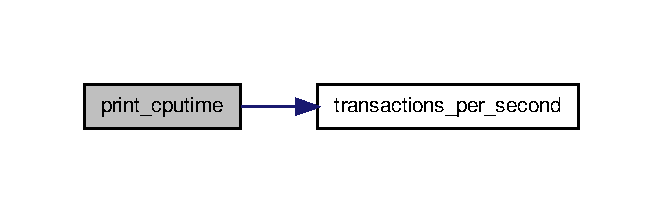
\includegraphics[width=318pt]{unit__test_8h_a2fdd86314c7b39ab4274a36655e833f1_cgraph}
\end{center}
\end{figure}



\section{unit\_\-test.h}

\begin{DoxyCode}
00001 \textcolor{comment}{/***************************************************************************}
00002 \textcolor{comment}{ *   Copyright (C) 2004-2011 by Patrick Audley                             *}
00003 \textcolor{comment}{ *   paudley@blackcat.ca                                                   *}
00004 \textcolor{comment}{ *   http://patrickaudley.com                                              *}
00005 \textcolor{comment}{ ***************************************************************************/}
00122 \textcolor{preprocessor}{#ifndef \_UNIT\_TEST\_H}
00123 \textcolor{preprocessor}{}\textcolor{preprocessor}{#define \_UNIT\_TEST\_H}
00124 \textcolor{preprocessor}{}
00125 \textcolor{preprocessor}{#ifdef UNITTEST}
00126 \textcolor{preprocessor}{}\textcolor{preprocessor}{#include <iostream>}
00127 \textcolor{preprocessor}{#include <vector>}
00128 \textcolor{preprocessor}{#include <sys/time.h>}
00129 \textcolor{preprocessor}{#include <sys/resource.h>}
00130 \textcolor{preprocessor}{#include <sys/types.h>}
00131 \textcolor{preprocessor}{#include <time.h>}
00132 
00133 
00134 \textcolor{keyword}{struct }rusage ruse;
00135 \textcolor{keyword}{extern} \textcolor{keywordtype}{int} getrusage();
00139 \textcolor{keyword}{inline} \textcolor{keywordtype}{double} cputime( \textcolor{keywordtype}{void} ) \{
00140   getrusage( RUSAGE\_SELF, &ruse );
00141         \textcolor{keywordflow}{return} ( ruse.ru\_utime.tv\_sec + ruse.ru\_stime.tv\_sec + 1e-6 * (ruse.ru\_ut
      ime.tv\_usec + ruse.ru\_stime.tv\_usec ) );
00142 \}
00149 \textcolor{keyword}{inline} \textcolor{keywordtype}{double} transactions_per_second( \textcolor{keywordtype}{double} run\_time, \textcolor{keywordtype}{unsigned} \textcolor{keywordtype}{long} transaction
      s ) \{
00150         \textcolor{keywordflow}{return} (\textcolor{keywordtype}{double})transactions / run\_time;
00151 \}
00158 \textcolor{keyword}{inline} \textcolor{keywordtype}{void} print_cputime( \textcolor{keyword}{const} \textcolor{keywordtype}{char}* msg, \textcolor{keywordtype}{double} run\_time, \textcolor{keywordtype}{unsigned} \textcolor{keywordtype}{long} transa
      ctions = 0 ) \{
00159         printf(\textcolor{stringliteral}{"  -> %s:  %7.3f seconds CPU time"}, msg, run\_time );
00160         \textcolor{keywordflow}{if}( transactions != 0 )
00161                 printf( \textcolor{stringliteral}{"  (%7.3f transactions/second)"}, transactions_per_second(
       run\_time, transactions ) );
00162         printf( \textcolor{stringliteral}{"\(\backslash\)n"} );
00163 \}
00164 
00166 \textcolor{keyword}{typedef} bool(*test_func)(void);
00168 \textcolor{keyword}{typedef} std::vector< test\_func > test\_vector;
00169 
00174 \textcolor{preprocessor}{#define UNIT\_TEST\_DEFINES \(\backslash\)}
00175 \textcolor{preprocessor}{  test\_vector * add\_test( test\_func x ) \{ \(\backslash\)}
00176 \textcolor{preprocessor}{    static test\_vector unit\_tests; \(\backslash\)}
00177 \textcolor{preprocessor}{    if( x != NULL ) unit\_tests.push\_back( x ); \(\backslash\)}
00178 \textcolor{preprocessor}{    return &unit\_tests; \(\backslash\)}
00179 \textcolor{preprocessor}{  \}}
00180 \textcolor{preprocessor}{}
00184 \textcolor{preprocessor}{#define DEFINE\_TEST(test\_name) bool unit\_test\_##test\_name (void)}
00185 \textcolor{preprocessor}{}
00191 \textcolor{preprocessor}{#define ADD\_TEST(test\_name) add\_test( &unit\_test\_##test\_name );}
00192 \textcolor{preprocessor}{}
00197 \textcolor{preprocessor}{#define UNIT\_TEST\_RUN( suite ) \(\backslash\)}
00198 \textcolor{preprocessor}{int main(void) \{ \(\backslash\)}
00199 \textcolor{preprocessor}{  bool result = true; \(\backslash\)}
00200 \textcolor{preprocessor}{  std::cout << "---[ " << suite << " ]--- " << std::endl;}
00201 \textcolor{preprocessor}{}
00205 \textcolor{preprocessor}{#define unit\_assert( msg, cond ) \(\backslash\)}
00206 \textcolor{preprocessor}{  std::cout << "  " << msg << ": " << std::flush; \(\backslash\)}
00207 \textcolor{preprocessor}{  if( !cond ) \{ std::cout << "FAILED" << std::endl; return false; \} \(\backslash\)}
00208 \textcolor{preprocessor}{  std::cout << "PASSED" << std::endl;}
00209 \textcolor{preprocessor}{}
00213 \textcolor{preprocessor}{#define unit\_pass() return true;}
00214 \textcolor{preprocessor}{}
00218 \textcolor{preprocessor}{#define unit\_fail() return false;}
00219 \textcolor{preprocessor}{}
00222 \textcolor{preprocessor}{#define UNIT\_TEST\_END \(\backslash\)}
00223 \textcolor{preprocessor}{  test\_vector *T = add\_test( NULL ); \(\backslash\)}
00224 \textcolor{preprocessor}{  for( unsigned short i = 0; i < T->size(); i++ ) \{ \(\backslash\)}
00225 \textcolor{preprocessor}{     bool testresult = (*(*T)[i])(); \(\backslash\)}
00226 \textcolor{preprocessor}{     if( result == true && testresult == false ) \{ result = false; \} \(\backslash\)}
00227 \textcolor{preprocessor}{  \} \(\backslash\)}
00228 \textcolor{preprocessor}{  return !result; \(\backslash\)}
00229 \textcolor{preprocessor}{\}}
00230 \textcolor{preprocessor}{}
00231 \textcolor{preprocessor}{#endif // UNITTEST}
00232 \textcolor{preprocessor}{}
00233 \textcolor{preprocessor}{#endif // \_UNIT\_TEST\_H}
\end{DoxyCode}

\chapter{Example Documentation}
\section{lru\_\-example.cpp}

\begin{DoxyCodeInclude}
\textcolor{preprocessor}{#include "lru_cache.h"}
\textcolor{preprocessor}{#include <string>}
\textcolor{preprocessor}{#include <iostream>}

\textcolor{keywordtype}{int} main(\textcolor{keywordtype}{void}) \{
        \textcolor{comment}{// Typedef our template for easy of readability and use.}
        \textcolor{keyword}{typedef} LRUCache<int,std::string> string\_cache\_t;
        
        \textcolor{comment}{// Instantiate a string cache with at most three elements.}
        string\_cache\_t *cache = \textcolor{keyword}{new} string\_cache\_t(3);
        
        \textcolor{comment}{// Insert data into the cache.}
        std::string quote\_1 = \textcolor{stringliteral}{"Number is the within of all things. -Pythagoras"};
        cache->insert( 4, quote\_1 );

        \textcolor{comment}{// Fetch it out.}
        std::cout << cache->fetch( 4 ) << std::endl;    
\}
\end{DoxyCodeInclude}
 
\printindex
\end{document}
